\sectionsansnumero{Introduction}
Ce document présente les différents aspects du projet ainsi que les problèmes auxquels nous avons été confrontés.
Les choix techniques sont présents à toutes les étapes, du cahier des charges (afin de le rendre réalisable et cohérent) à la mise en œuvre finale.
Il présente aussi dans les grandes lignes les étapes de validation de la carte telles qu'elles sont envisagées.
Ce document est donc structuré en quatre parties~:
\begin{itemize}
	\item La première partie présente le contexte de ce projet ainsi que ses objectifs pédagogiques
	\item La deuxième partie présente le cahier des charges qui a été à l'origine de ce projet personnel
	\item La troisième partie détaille les choix techniques liés au matériel
	\item La quatrième partie détaille les choix des composants logiciels sélectionnés afin d'exploiter cette carte
\end{itemize}
    
\section{Contexte}
Ce projet est réalisé dans le cadre du Projet de Réalisation Technologique de 4\ieme{} année du département de Génie Électrique de l'INSA de Lyon.
Il a pour objectif de développer des compétences pratiques dans la réalisation d'un système électronique embarqué.
Il a fait l'objet d'une réflexion en amont afin d'identifier les objectifs et a ensuite été proposé en projet de PRT avec des objectifs atteignables dans l'état actuel de nos connaissances.
    
\section{Cahier des Charges}
L'objectif est de réaliser une carte de développement construite autour d'un ARM Cortex-M4 dans le but d'y utiliser un système GNU/Linux.
La première contrainte physique qui en découle est la nécessité d'une RAM externe (la RAM interne de 256Ko étant trop petite pour faire tourner un tel système).
Il faut également de la mémoire Flash de stockage externe (la mémoire Flash interne de 2Mo est tout juste capable de stocker un système de base composé d'un bootloader, d'un noyau et de BusyBox \autocite{BusyBox}).
Afin de rendre le projet plus intéressant du point de vue des applications possibles du résultat, les périphériques suivants ont été implémentés:
\begin{itemize}
	\item Ecran LCD couleur 480x272
	\item USB On-The-Go (hôte et esclave)
	\item UART
	\item Un certain nombre de \glspl{GPIO}, également utilisables pour d'autres usages tels que un bus I2C
\end{itemize}

Le microcontrôleur de cette carte est un ARM Cortex-M4 produit par STMicroelectronics, le STM32F429ZI.
Un portage de uClinux 2.6.33 (février 2010) sur cette plate-forme est disponible et maintenu par la société Emcraft, ce qui a entre autres poussé au choix de ce microcontrôleur.

\section{Hardware}
\subsection{Microcontrôleur}
\subsubsection{Choix du microcontrôleur}
De nombreux microcontrôleurs sont disponibles aujourd'hui et se confrontent sur l'arène de l'électronique embarquée, on peut citer notamment les familles suivantes :
\begin{itemize}
	\item Atmel AVR (8-bit), AVR32 (32-bit)
	\item Microchip Technology PIC, (8-bit PIC16, PIC18, 16-bit dsPIC33 / PIC24), (32-bit PIC32)
	\item Texas Instruments MSP430 et C2000
	\item Processeurs/microcontrôleurs à base d'ARM
\end{itemize}
            
Un acteur tire son épingle du jeu et se démarque particulièrement des autres : ARM.
ARM est une société britannique spécialisée dans le développement d'architectures 32 bits de type RISC. 
C'est une entreprise \angl{fabless} dont le modèle économique particulier de la microélectronique : la conception de \gls{IP}.
Ainsi il n'est pas possible d'acheter un processeur/microcontrôleur directement à ARM comme c'est le cas pour Intel, des licences sont attribuées à d'autres fabricants de semi-conducteurs qui proposent donc des puces basées sur la propriété intellectuelle ARM dans leurs catalogues.
Les cœurs ARM sont le plus souvent intégrés au sein de \gls{SoC} complets.
Ils sont très présents dans les systèmes embarqués (téléphone mobile, console portable, tablette électronique).
En 2010, ARM était présent dans plus de 95\% des smartphones, 10\% des ordinateurs portables et 35\% des télévisions connectées et set-top box. \autocite{ARMMS}
En 2014, plus de 50 milliards de chipsets à base d'ARM ont été produits. ARM vise aujourd'hui à s'implanter sur le marché des ordinateurs personnels et des serveurs, notamment avec des projets tels qu'Euroserver \autocite{Euroserver}.
Les perspectives de croissances sont prometteuses.
            
Au vu des données ci-dessus, il parait évident que la connaissance des technologies ARM devient de plus en plus importante pour un ingénieur génie électrique aujourd'hui. 
C'est la raison principale pour laquelle nous avons choisi de travailler sur un ARM.

ARM a commencé à développer une gamme de Cortex-M, depuis 2003. 
Ce sont des microcontrôleurs relativement simples (en opposition aux Cortex A par exemple), ils sont facilement intégrables pour les raisons citées en introduction. \\
            
\begin{center}
	\begin{tabular}{|c|c|}
		\hline
		Année d'annonce & Core       \\
		\hline
		2004             & Cortex-M3  \\
		2007             & Cortex-M1  \\
		2009             & Cortex-M0  \\
		2010             & Cortex-M4  \\
		2012             & Cortex-M0+ \\
		2014             & Cortex-M7  \\
		\hline
	\end{tabular}
\end{center}
            
Dans la série des Cortex-M, notre choix s'est porté sur un Cortex-M4 car c'est l'un des plus puissants de la gamme, derrière les Cortex-M7.
Il implémente l'architecture ARM v7-M.
Ce qui le différencie particulièrement des autres Cortex inférieurs est que le M4 dispose d'instructions de \gls{DSP} et d'une \gls{FPU} optionnelle.
Conceptuellement, un Cortex-M4 est un Cortex-M3 avec ces deux éléments en plus. Un Cortex-M4 embarquant ledit FPU est nommé Cortex-M4\textbf{F}\\
            
De nombreux fabricants proposent aujourd'hui des microcontrôleurs basés sur un ARM Cortex-M4/M4F, on peut citer :
\begin{itemize}
	\item Atmel SAM4L, SAM4N, SAM4S, SAM4C (dual core), SAM4E, SAMG
	\item Freescale Kinetis K, W2
	\item NXP LPC4000, LPC4300 (dual core, Cortex-M4F + one Cortex-M0)
	\item STMicroelectronics STM32 F3, F4, F7 (nouvelle famille basée sur le coeur ARM Cortex M7 dotée de caches)
	\item Texas Instruments LM4F, TM4C et plus récemment le MSP432
\end{itemize}
            
Ces chipsets se valent pratiquement tous et proposent les mêmes fonctionnalités.
Le STM32F429ZI a été retenu, car c'est l'un des moins chers du marché (12,54 €) à être cadencé à 180 MHz, et supporter les périphériques que l'on souhaite implémenter (SDRAM, NOR Flash, LCD, USB). 
De plus, la documentation proposée par ST est relativement exhaustive (datasheets, notes d'applications abondantes) et le portage de uClinux déjà réalisé.
            
Autre avantage de ce chipset : une carte d'évaluation existe déjà embarquant une grande partie des périphériques que nous souhaitons implémenter. 
Nous avons acquis cette carte d'évaluation en début du projet pour paralléliser les développements hardware et software.
            
\subsubsection{Présentation du STM32F429ZI}
Le microcontrôleur choisi est donc le STM32F429ZI qui est donc un Cortex-M4F cadencé à 180 MHz embarquant un \gls{DSP} et une \gls{FPU}.
Il dispose de 2MB de Flash interne organisée en 2 banques permettant un \angl{read-while-write}, 256KB de SRAM, un \gls{FMC} permettant l'interfaçage du MCU avec différents types de mémoires externes : SRAM, PSRAM, SDRAM/LPSDR SDRAM, Compact Flash/NOR/NAND, un contrôleur LCD parallèle permettant de driver des écrans en RGB565/666, 3×12-bit, 2.4 MSPS ADC, 2×12-bit DAC, un contrôleur DMA 16-canaux, 17 Timers. \\
En termes de périphériques d'IO, le STM32F429ZI dispose de 4 entrées pour encodeurs, 3xI2C, 4 USARTs/4 UARTs, 6 SPIs avec 2 interfaces I2S full-duplex pour l'audio, 1 SAI (serial audio interface), 1 contrôleur USB 2.0 full-speed \footnote{USB 2.0 full-speed : 12 Mbit/s.}  device/host/OTG avec un PHY embarqué et 1 contrôleur USB 2.0 high-speed/full-speed \footnote{USB 2.0 high-speed : 480 Mbit/s.}device/host/OTG avec DMA dédié à utiliser avec un \gls{PHY} externe (interface \gls{ULPI} avec ce dernier), 1 contrôleur 10/100 Ethernet MAC avec DMA dédié à utiliser avec un \gls{PHY} externe (interface \gls{MII/RMII} avec ce dernier).\\
Deux interfaces de debug sont implémentées : le \gls{JTAG} et le \gls{SWD}.
      
\subsection{Mémoire vive externe (RAM)}
\subsubsection{Principe de fonctionnement}
Il y a deux technologies de fabrication des RAM : statiques et dynamiques. \\
\begin{itemize}
	\item La SRAM ou RAM Statique est la plus ancienne. 
	      Les bits y sont mémorisés par des bascules électroniques dont la réalisation nécessite six transistors par bit à mémoriser. 
	      Les informations y restent mémorisées tant que le composant est sous tension et n'ont pas besoin d'être rafraîchies.
	      Chaque bit d'une SRAM est formé par une bascule (latch) constituée de 4 à 6 transistors. \\
	      Le bascule RS comporte : deux entrées notées R (Reset) et S (Set) et deux sorties désignées par Q et -Q qui ont des valeurs inverses.
	      	                  
	      \begin{center}
	      	\begin{tabular}{|l|c|r|}
	      		\hline
	      		S & R & Sortie Q   \\
	      		\hline
	      		0 & 0 & Inchangée \\
	      		\hline
	      		0 & 1 & Q = 0      \\
	      		\hline
	      		1 & 0 & Q = 1      \\
	      		\hline
	      		1 & 1 & -          \\
	      		\hline
	      	\end{tabular}
	      \end{center}
	      	      
	      La SRAM est très rapide et est pour cette raison le type de mémoire qui sert aux mémoires cache.
	      Mais compte tenu du nombre de transistors nécessaires pour stocker un bit de données, son coût est prohibitif et sa densité faible. \\
	\item La DRAM pour RAM dynamique est plus simple à réaliser que la SRAM. 
	      Cela permet de faire des composants de plus haute densité et dont le coût est moindre. 
	      Chaque bit d'une DRAM est mémorisé par une charge électrique stockée dans un petit condensateur (dont la capacité est de l'ordre de la dizaine de fF). 
	      Ce dispositif offre l'avantage d'être très peu encombrant, mais a l'inconvénient de ne pas pouvoir garder l'information longtemps. 
	      Le condensateur se décharge au bout de quelques millisecondes (ms). 
	      Pour ne pas perdre le bit d'information qu'il contient, il faut un dispositif qui lit la mémoire et qui la réécrit de suite pour recharger les condensateurs. 
	      Ces RAM sont dites dynamiques, car cette opération de rafraîchissement ou de lecture doit être répétée régulièrement (64ms ou 16ms dans le domaine de l'automobile). \\
	      Il nous a semblé important de bien comprendre le principe de fonctionnement des DRAM avant de nous lancer dans son implantation sur notre carte. \\
	      	                  
	      \begin{figure}[H]
	      	\begin{center}
	      		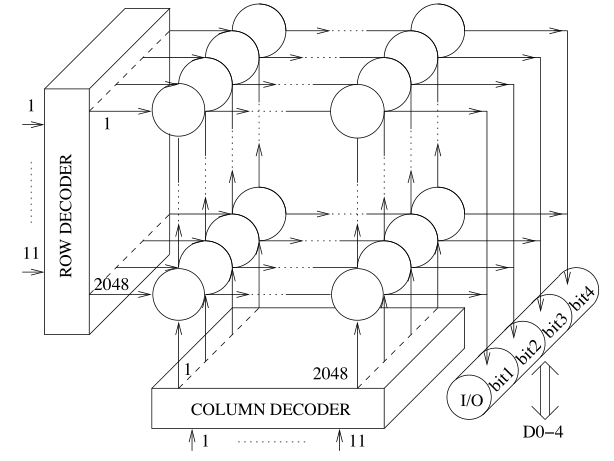
\includegraphics{DRAM_Structure}
	      	\end{center}
	      	\caption{Organisation d'une DRAM}
	      \end{figure}
	      	                  
	      La figure 1 est une représentation simplifiée de la structure d'une DRAM.
	      Chaque cercle représente une cellule mémoire, les lignes sortant des \angl{decoders} sont utilisées pour sélectionner la cellule mémoire à activer et les lignes sortant des cellules mémoires sont utilisées pour transférer les données stockées dans le buffer I/O.
	      La DRAM représentée ici fait 2048x2048x4=16 MBits. \\
	      	                  
	      \begin{figure}[H]
	      	\begin{center}
	      		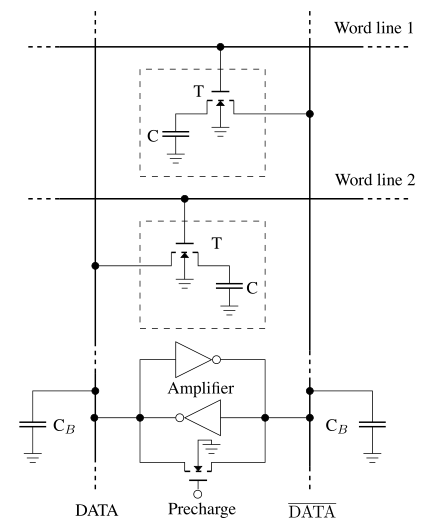
\includegraphics{DRAM_Memory_Cell}
	      	\end{center}
	      	\caption{Cellule mémoire d'une DRAM}
	      \end{figure}
	      	                  
	      Chaque cellule mémoire a un condensateur enregistrant la donnée sous forme d'une charge électrique et un transistor d'accès agissant comme interrupteur pour sélectionner le condensateur.
	      La grille du transistor d'accès est connectée à la \textit{word line}. Une cellule mémoire contient autant de \textit{word line} que de lignes mémoire.
	      Les \angl{bit line} sont connectées à DATA et \#DATA. Il y a autant de \angl{bit lines} que de colonne mémoires. \\
	      Avant d'accéder accès à la mémoire, le contrôleur de la DRAM effectue une opération dite de précharge : les \angl{bit line} complémentaires sont portées à VCC/2.
	      Ce mécanisme sert à gagner du temps lors des accès mémoires. Le contrôleur effectue ensuite une opération dite d'égalisation : les \angl{bit line} sont court-circuitées avec un transistor pour être exactement au même potentiel.
	      Le temps nécessaire à la précharge et l'égalisation est appelée \angl{RAS precharge time} et le contrôleur ne peut accéder aux données qu'une fois ces opérations finies. \\
	      Quand le contrôleur veut accéder à une cellule mémoire, il fournit le signal \angl{row address} pour sélectionner la ligne, ce signal passe par le \angl{row buffer} puis est transféré au \angl{row decoder}.
	      Ce dernier décode l'adresse de la ligne et active la \angl{word line} correspondante à la ligne à laquelle on désire accéder. 
	      A ce niveau, tous les transistors d'accès de la ligne sélectionnée sont passants.
	      Les charges contenues dans les condensateurs de stockage s'écoulent vers les condensateurs \(C_B\). \\
	      Le problème est que les valeurs des condensateurs de stockage sont plus faibles que les capacités des \angl{bit line} donc le potentiel de ces dernières varie peu (de l'ordre de la centaine de mV seulement) et dans un intervalle de temps très court.
	      Pour régler ce problème, des amplificateurs ont été rajoutés.
	      Si le condensateur de stockage est vide, le potentiel de la \angl{bit line} correspondante décroit, si le condensateur de stockage est chargé, le potentiel de la \angl{bit line} croît.
	      L'amplificateur amplifie la différence de potentiel entre la paire de \angl{bit line}.
	      Dans le premier cas, le potentiel de la \angl{bit line} connectée au condensateur est mis à la masse et l'autre à VCC.
	      Dans l'autre cas, c'est l'inverse qui se passe. \\
	      Sans préchargement ni égalisation, l'amplificateur devrait porter augmenter/diminuer le potentiel de VCC au lieu de VCC/2. \\
	      Les signaux amplifiés sont transférés à l'\angl{IO gate block}. 
	      Le \angl{column decoder} décode l'adresse de la colonne à laquelle on souhaite accéder et transfère finalement le bit choisi au bloc IO. \\
	      On notera que l'accès aux données est destructif puisque le condensateur se vide.
	      C'est là qu'intervient le condensateur \(C_B\).
	      Nous avons initialement copié la valeur originale dedans avant l'accès mémoire. \\
	      L'accès à une seule cellule mémoire entraîne le rafraîchissement de la ligne entière. \\
\end{itemize}
\subsubsection{Solution retenue}
Les SDRAM sont des variantes synchrones des DRAM fonctionnant sur le même principe.
Elles sont économiques, d'une plus grande densité (5 à 10 fois que les SRAM) mais sont également plus lentes. \\
La grande majorité des SDRAM vendues aujourd'hui embarquent des contrôleurs gérant les aspects physiques liés au rafraîchissement, préchargement, égalisation etc. facilitant de fait l'intégration de ce type de mémoires. 
A titre indicatif, le prix d'une SRAM de 16 Mbit (1M X 16 bit) est de 12€ sur Farnell contre 2,7€ pour une SDRAM de même capacité. \\
La référence retenue est donc une Micron MT48LC32M8A2P-7E \autocite{micron:MT48LC32M8A2P7E} de 256 Mbit cadencée à 133 MHz et de boîtier TSOP2 54 broches. Elle s'organise en 4 banques internes de 8Mx8x4.\\        	
    
\subsubsection{Interface des SDRAM}
L'interface des SDRAM est standardisée par le JEDEC \autocite{JEDEC}.
Ceci permet une bonne interopérabilité des différentes mémoires avec les différents contrôleurs.
Les signaux sont les suivants \autocite{micron:MT48LC32M8A2P7E}~:
\begin{itemize}
	\item CLK : horloge de synchronisation
	\item CKE : Clock Enable, permet d'entrer dans un mode de basse consommation
	\item CS\# : Chip Select, actif bas, permet d'activer la SDRAM pour signifier qu'elle doit lire une commande. Ceci permet de partager bus de donnée et d'adresse avec d'autres mémoires, comme c'est le cas avec le \gls{FMC} (mémoire SDRAM et NOR)
	\item CAS\#, RAS\#, WE\#: Column Address Strobe, Row Address Strobe, Write Enable: commande permettant respectivement de sélectionner une colonne, une ligne, et enfin d'informer d'un accès en lecture (WE haut) ou en écriture (WE bas).
	\item BA[1:0] : sélection de la banque interne sur laquelle s'appliqueront les commandes
	\item A[12:0] : bus d'adresse
	\item DQ[8:0] : bus de données                
\end{itemize}

Lors de l'accès à une banque donnée, le contrôleur envoie une commande de préchargement afin de désélectionner la ligne précédemment sélectionnée si ce n'est pas la bonne.
Il envoie ensuite une commande d'activation d'une ligne (RAS\#) en précisant son adresse sur le bus d'adresse, en même temps que la banque interne désirée au bout d'un temps $t_{RP}$.
Au bout d'un nombre de cycles $t_{RCD}$, une commande CAS\# est envoyée, avec l'adresse de la colonne sur le bus d'adresse.
Au bout d'un temps $t_{CL}$, les données sont accessibles sur le bus de donnée.
Une écriture nécessite l'usage du signal WE\#.
		
\begin{figure}[H]
	\begin{center}
		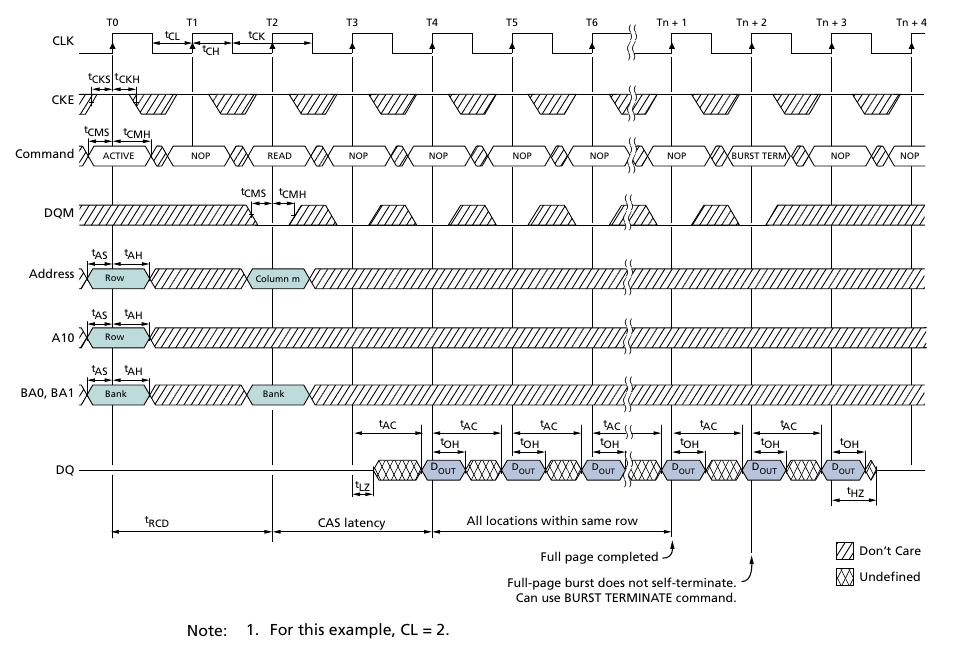
\includegraphics[scale = 0.6]{SDRAM_read_timing_Micron}
	\end{center}
	\caption{Chronogramme d'un accès en lecture à la SDRAM Micron choisie \autocite{micron:MT48LC32M8A2P7E}}
\end{figure}
        
        
En plus de ce fonctionnement de base, les SDRAM possèdent généralement plusieurs modes.
En effet, la SDRAM est capable de fournir plus qu'un mot lors de la lecture d'une colonne sélectionnée.
Ceci est appelé un \angl{burst}, dont la taille est configurable à l'initialisation de la SDRAM.

\subsection{Mémoire de stockage de masse (Flash)}
Afin de pouvoir stocker le \angl{firmware} de notre carte, il est nécessaire de rajouter de la mémoire de stockage de masse externe, car la Flash interne du microcontrôleur n'est pas suffisante (2Mo).
        
\subsubsection{Comparatif}		
Deux familles de mémoire Flash sont disponibles~: les NOR et les NAND.
            
Les NOR permettent un accès mot par mot, alors que les NAND utilisent un protocole plus complexe et ne permettent d'accéder qu'à des pages.
La NOR permet donc l'\gls{XIP}, car le cœur du microcontrôleur peut accéder aux instructions mot à mot, de manière transparente grâce au contrôleur mémoire \gls{FMC} qui est un esclave \gls{AHB}.
            
En contrepartie, les NAND ont une meilleure densité et sont donc moins chères.
Les NAND possèdent également un système de stockage de métadonnées associées à chaque page permettant de marquer les pages qui ne sont plus utilisables ainsi que des codes correcteurs d'erreur.
            
En effet, toutes les mémoires flash sont sensibles à un phénomène d'usure compté en nombre de cycles écrasement/écriture qui s'élève généralement de 10 000 à 100 000 \footnote{\url{http://en.wikipedia.org/wiki/Flash_memory}}.
Cette fonctionnalité permet de relâcher les contraintes sur la qualité de production, et donc de baisser les prix, en augmentant la difficulté d'utilisation.
            
Une particularité des mémoires Flash est qu'une écriture ne peut que transformer un bit 1 en bit 0.
Pour transformer un bit 0 en bit 1, il faut écraser un secteur, ce qui se fait avec généralement une granularité moins fine que les opérations de lecture dans le cas de la NOR.
            
La mémoire retenue est une mémoire NOR Spansion S29GL256P90TFIR20 de 32Mo avec un bus de donnée de 16 bits.
Ce choix permet d'utiliser l'\gls{XIP} qui évite de copier le code des programmes en RAM avant l'exécution, permettant donc de gagner une place notable pour les données.
Le bus de 16 bit est particulièrement adapté sur cette plate-forme, car les instructions encodées en  \gls{THUMB} font généralement 16 bits.
Ceci permet donc de lire une instruction en un cycle de lecture de la NOR.
            
\subsubsection{Interface des NOR}
L'interface des mémoires NOR est également standardisée par le JEDEC \autocite{JEDEC}.
Les signaux suivants sont nécessaires au fonctionnement de la NOR \autocite{spansion:S29GL256P}~:
\begin{itemize}
	\item A25–A0 : Bus d'adresse. Une adresse est associée à un mot de 16 bits et non à un octet
	\item DQ15–DQ0 : Bus de données 16 bits
	\item CE\# : Chip Enable, actif bas, permet de sélectionner la NOR car elle partage le bus d'adresse et de données avec la SDRAM
	\item WE\# : Write Enable, permet de spécifier une commande d'écriture
	\item BYTE\# : Sélectionne la largeur du bus de données à utiliser (16 bits dans notre cas)
	\item RESET\#
\end{itemize} 

\begin{figure}[H]
	\begin{center}
		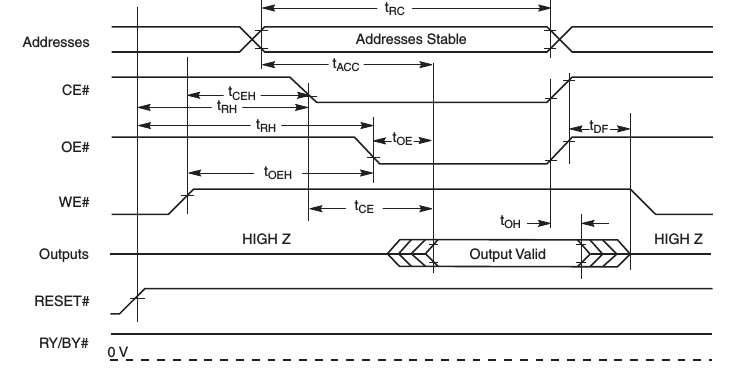
\includegraphics[scale = 0.6]{NOR_read_timing_Spansion}
	\end{center}
	\caption{Chronogramme d'un accès en lecture à la NOR Spansion choisie \autocite{spansion:S29GL256P}}
\end{figure}
        
L'écrasement d'un secteur est une opération longue et sa durée peut être variable d'une puce à l'autre.
Il est donc nécessaire de prévenir le processeur lorsque cette opération est finie.
L'interface \gls{CFI} permet à un pilote générique d'interroger la mémoire NOR afin de récupérer les valeurs maximales des temporisations d'écrasement.
Ainsi, un pilote pour une NOR compatible \gls{CFI} n'aura pas besoin d'être recodé pour chaque mémoire NOR, uniquement pour chaque contrôleur de mémoire.

\subsection{Périphériques et interfaces}
\subsubsection{IHM - Écran LCD}       
L'écran que nous allons utiliser pour ce projet a été récupéré au ClubElek sur d'anciennes cartes de développement de TI (AM335x Starter Kit). 
Il s'agit d'un écran LCD fabriqué par Newhaven Display, \verb$NHD-4.3-480272MF-ATXI#-T-1$ \autocite{newhaven:NHD}. 
C'est un écran LCD de résolution 480x272, affichant jusqu'à 16.7M couleur. 
Il est également équipé d'une dalle tactile résistive et d'un rétroéclairage intégré. 
Le driver implémenté sur l'écran est un Orise OTA5180A supportant que le RGB888 \autocite{orise:OTA5180A}. 
L'écran est autosuffisant : il suffit de lui fournir une tension de 3V3 pour l'alimentation, une tension de 21V pour le rétroéclairage et des signaux vidéos avec les bons timings. 
Toute l'implémentation hardware du driver est déjà réalisée par Newhaven Display.
Le protocole vidéo utilisé est un protocole LCD parallèle relativement standard. Les différents signaux à fournir sont :
        
\begin{itemize}
	\item PLCK : horloge de synchronisation
	\item DISP : allumage/extinction de l'écran
	\item HSYNC : signal de synchronisation de lignes
	\item VSYNC : signal de synchronisation de trames 
	\item DE : sélection de l'activation des données
	\item R[7:0] : données de couleur rouge
	\item G[7:0] : données de couleur verte 
	\item B[7:0] : données de couleur bleue
\end{itemize}
            
La difficulté de ce genre d'interfaces n'est pas tant l'intégration hardware (l'horloge vidéo est à 9 MHz) c'est plutôt les drivers software générant les bons timings vidéos.
Le boîtier 144 broches de notre microcontrôleur a cependant posé un problème: en effet, certains signaux nécessaires au fonctionnement de la mémoire NOR utilisent les mêmes broches que des bits de poids faible des bus de couleur de l'écran (signaux R, G et B).
Il a donc été décidé de relier ces bits de poids faibles à la masse afin de les utiliser pour la NOR.
On obtient alors une configuration RGB666.
            
Ces timings sont assez communs dans le monde de la vidéo (CVBS, MIPI, ...).
Il s’agit des \angl{Front porch}, \angl{Back porch} horizontaux et verticaux.
La spécification de ces timings se trouve dans la datasheet de l'Orise OTA5180A \autocite{orise:OTA5180A}.
            
\begin{figure}[H]
	\begin{center}
		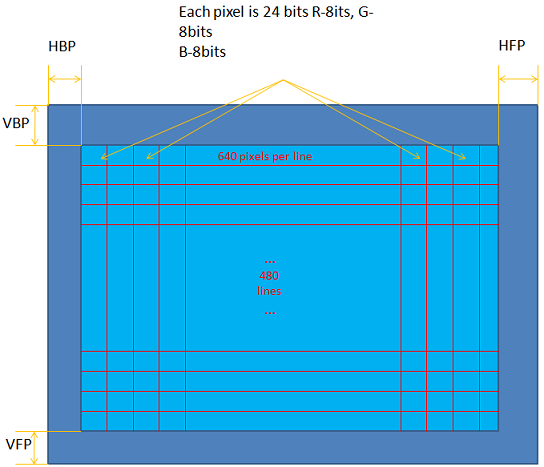
\includegraphics[scale = 0.5]{Timings_Video}
	\end{center}
	\caption{Timings vidéos d’une trame de 640x480}
\end{figure}
            
Ces paramètres sont un héritage des vieux standards de télévision que sont le PAL et le NTSC.
À l’époque des télévisions à tube cathodique, c’est un faisceau d’électrons qui balaie l’écran et, en frappant une surface recouverte de matériaux phosphorescents, génère une lumière sur l’écran. 
La déviation de ce faisceau était faite par un champ magnétique généré par des bobines. 
Deux signaux électriques sont principalement appliqués pour se faire :
\begin{itemize}
	\item Un signal commandant le balayage horizontal («en x»), sur les bobines situées au-dessus et en dessous du faisceau;
	\item Un signal commandant le balayage vertical («en y»), sur les bobines situées à gauche et à droite du faisceau.
\end{itemize}
Les temps de \angl{blanking} ont été introduits pour synchroniser le faisceau sur la partie dite «active» de l’écran. 
Ainsi le \angl{Vertical Blanking Interval} ou \angl{Vertical Front/Back Porch} ont été introduits pour laisser le temps au faisceau de remonter en haut de l’écran à la fin d’une trame. 
Il en va de même pour l'\angl{Horizontal Blanking Interval} ou \angl{Horizontal Front/Back Porch}.
Ces réglages représentent une des parties délicates à parfaire avant de pouvoir afficher
une image correcte.

\begin{figure}[H]
	\begin{center}
		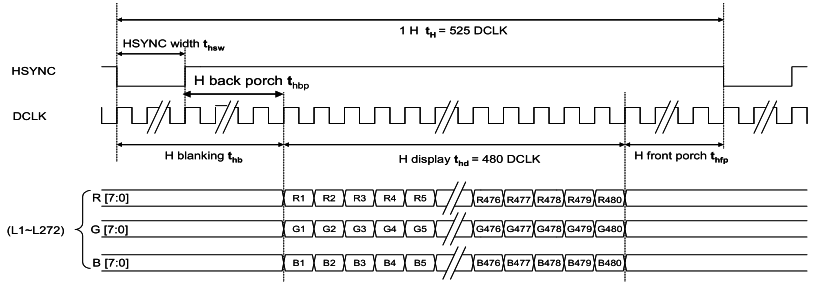
\includegraphics[scale = 0.6]{Timings_Video_Orise}
	\end{center}
	\caption{Timings vidéos LCD}
    \source{Datasheet du contrôleur LCD Orise OTA5180A \autocite{orise:OTA5180A}} 
\end{figure}

\subsubsection{M2M}       
\begin{itemize}
	\item UART:
	      Des signaux d'UART ont été routés sur des \angl{headers} pour pouvoir communiquer en série avec la carte.
	      Cette communication série pourra servir au debug ainsi qu'à de la communication \angl{Machine to machine}.
	\item \glspl{GPIO}~:
	      20 \glspl{GPIO} ont été laissés à l'utilisateur pour être utilisées comme \glspl{GPIO} ou d'autres bus tels qu'I2C. 
\end{itemize}          	


\subsection{Outils utilisés}
\subsubsection{STM32CubeMX}
Le STM32CubeMX \autocite{STM32CubeMX} est un outil fourni par ST pour faciliter et accélérer les développements des produits embarquant un MCU STM32.
C'est un outil permettant de générer le code d'initialisation en C en utilisant l'interface graphique. 
Plusieurs fenêtres sont disponibles : l’assistant « brochage » facilite l’affectation des broches pour éviter les conflits grâce à un solveur de conflits embarqué ; l’assistant « arbre d’horloge » attribue les horloges et exécute la validation dynamique ; l’assistant « périphériques et middleware » pour éviter tout paramètre non utilisable/conflit ; et l’assistant « consommation d’énergie » qui permet d'estimer la consommation de MCU et les périphériques configurés.
Il a grandement servi lors du développement hardware pour faire le \angl{mapping} des signaux en sortie/entrée du MCU et à s'assurer facilement et rapidement qu'il n'existe pas de conflit entre les différentes fonctionnalités associées à chaque broche.
        
\begin{figure}[H]
	\begin{center}
		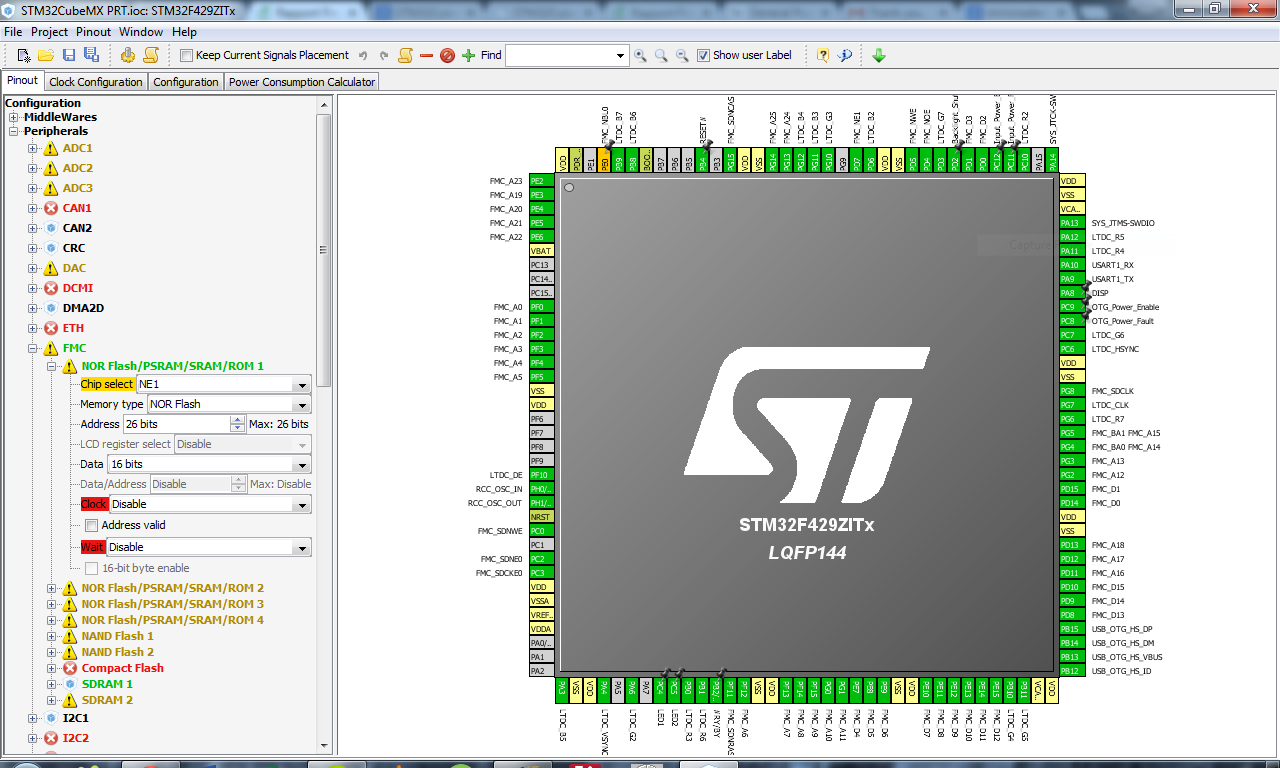
\includegraphics[scale = 0.45]{STM32CubeMX}
	\end{center}
	\caption{Interface de STM32CubeMX}
\end{figure}
            
\subsubsection{Altium}
Altium Designer \autocite{Altium} est un logiciel de conception assistée par ordinateur pour systèmes électroniques. Altium Designer propose des fonctions de \autocite{AltiumWiki}:
\begin{itemize}
	\item Saisie de schémas
	\item Simulation (basée sur Xspice)
	\item Conception/routage de circuits imprimés, capture des schémas, gestion des bibliothèques de composants, routage, génération des fichiers de fabrication \gls{Gerber}
	\item Programmation de FPGA et microprocesseurs/microcontrôleurs
	\item Interfaçage avec des logiciels de CAO mécanique (SolidWorks par ex.) permettant de faciliter l'intégration de l'électronique dans la mécanique
\end{itemize}
            
Nous avons choisi d'utiliser ce logiciel plutôt qu'une autre (Eagle, Allegro, KiCad, etc.) parce que c'est celui que nous utilisons au ClubElek et que nous savons utiliser.
            
\subsubsection{SVN}
Afin d'héberger les différents documents concernant le projet ainsi que les schémas électriques, un dépôt SVN a été créé sur la plate-forme Assembla \autocite{Assembla}.
Un compte gratuit correspondant aux prestations normalement payantes nous a gracieusement été offert par l'équipe d'Assembla.
Ce dépôt SVN permet de versionner tous les fichiers, sans risques de perdre ou d'écraser des modifications, et il permet aussi de synchroniser facilement entre nos ordinateurs et de manière déterministe (contrairement à Dropbox ou encore Google Drive qui ne sont pas vraiment adapté car on ne choisit pas l'instant de synchronisation, ce qui amène des problèmes).
De plus, SVN est intégré à Altium, nous pouvons gérer le versionnement directement depuis celui-ci.
	
\subsection{Mise en œuvre du PCB}
\subsubsection{Schématique}
Nous avons commencé par faire les schémas de la carte.
Pour garder de la lisibilité, nous n'avons pas mis tous les schémas sur une feuille A0.
Nous avons découpé les pages de schémas en blocs logiques s'inspirant fortement du diagramme que nous avons initialement défini. \\
Altium dispose d'outils puissants permettant de faire ce genre de schématique en utilisant différents types de connecteurs pour relier les signaux entre eux \autocite{AltiumMultiSheet} (\angl{Net Label}, \angl{Port}, \angl{Sheet Entry}, etc.).
        
\begin{figure}[H]
	\begin{center}
		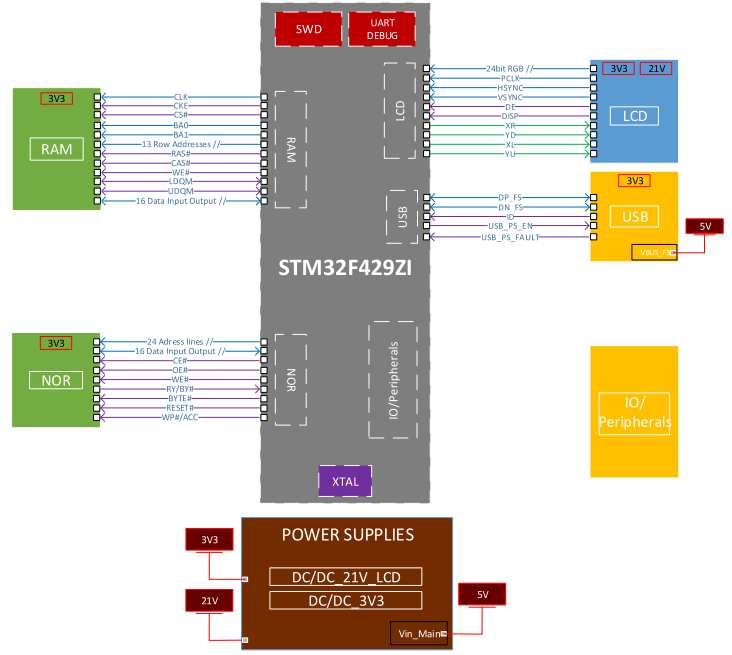
\includegraphics[scale = 0.7]{Bloc_Diagram}
	\end{center}
	\caption{Schéma-bloc de la carte}
\end{figure}
        
        
Revoyons page par page de la schématique (page \pageref{sec:AnnexeSchematic}) les points importants :
\begin{itemize}
	\item \hyperlink{Schematic.2}{Alimentations} :
	      nous avons choisi d'alimenter notre carte à partir d'une alimentation USB standard délivrant du 5V (du même genre qu'on utilise pour charger nos smartphones).
	      Ce choix nous évite d'avoir besoin d'une alimentation stabilisée pour générer les tensions nécessaires à la carte et d'utiliser un convertisseur AC/DC pour passer de la tension secteur à un 3V3 stabilisé. \\
	      Nous avons besoin de deux tensions différentes sur notre carte : une tension de 3,3V pour alimenter tous les circuits numériques que nous utilisons et une tension de 21V pour alimenter les LEDs de rétroéclairage d'écran. \\
	      Nous avons fait la somme des courants consommés par chaque \glspl{IC} dans le pire des cas à 85°C, nous arrivons à un pire cas de 580 mA sur l'alimentation 3,3V.
	      Nous choisisons donc d'utiliser un convertisseur Buck pour faire la conversion 5V/3,3V. \\
	      Nous choisisons d'utiliser un Buck de TI, le LMR10510.
	      Il dispose de caractéristiques parfaitement adaptées à nos besoins :
	      \begin{itemize}
	      	\item \angl{Input voltage range of \textbf{3V to 5.5V}}
	      	\item \angl{Output voltage range of \textbf{0.6V to 4.5V}}
	      	\item \angl{Output current \textbf{up to 1A}}
	      	\item \angl{\textbf{1.6-MHz} Switching Frequency}
	      	\item \angl{Low shutdown Iq, \textbf{30 nA} typical}
	      	\item \angl{Internal soft-start}
	      	\item \angl{Internally compensated}
	      	\item \angl{\textbf{Thermal shutdown}}
	      \end{itemize}
	      De plus le boîtier de ce Buck est un SOT23 tout à fait soudable manuellement.
	      Le LMR10510 est proposé à 1,08€ sur Farnell et TI fournit des samples gratuitement. \\
	      La fréquence relativement élevée de découpage de ce Buck à 1,6 MHz permet de réduire la taille de l'inductance ce qui permet une plus grande intégration de la carte.
          
	      Le dimensionnement de l'inductance, la capacité et la diode de sortie a été fait en utilisant une feuille Excel que nous avons crée.
	      Les formules utilisées proviennent de la datasheet et des cours que nous avons eu. \\
	      Les valeurs calculées sont les suivantes :
	      	             
	      \begin{center}
	      	\begin{tabular}{|c|c|c|}
	      		\hline
	      		Rapport cyclique & Valeur d'inductance & Capacité de sortie \\
	      		\hline
	      		70\%             & 2,19 nH             & 40 nF               \\
	      		\hline
	      	\end{tabular}
	      \end{center}
	      	                  
	      Pour la diode, nous choisisons une diode Schottky pour sa tension directe faible et ses temps de commutation faible adaptée adaptée à notre fréquence de découpage.
	      Nous ferons attention également à ce que sa tension de blocage inverse soit au moins de 3,3V. \\
	      	                  
	      Nous utilisons les valeurs proposées par la datasheet pour une tension d'entrée de 5V, une tension de sorte de 3,3V et un courant de sortie moyen de 1A :
	      	                  
	      \begin{center}
	      	\begin{tabular}{|c|c|c|}
	      		\hline
	      		Valeur d'inductance & Capacité de sortie \\
	      		\hline
	      		2,2 uH              & 22 uF               \\
	      		\hline
	      	\end{tabular}
	      \end{center}
	      	                  
	      Nous remarquons que les valeurs de la capacité et de l'inductance sont largement supérieures à celles que nous avons calculées.
	      Cela impacte positivement les performances du système puisque ça a pour effet de diminuer le courant de \angl{ripple}.
	      Nous estimons que celui-ci sera de quelques mV.
	      	                  
	      Pour générer la tension de 21V, nous utilisons un Boost.
	      Nous estimons le courant de charge à 40 mA dans le pire des cas. \\
	      Nous choisisons pour pratiquement les mêmes raisons que le Buck d'utiliser le LM27313 de TI. Ses caractéristiques sont les suivantes : 
	      \begin{itemize}
	      	\item \angl{Input Voltage Range \textbf{(2.7 V to 14 V)}}
	      	\item \angl{\textbf{1.6-MHz} Switching Frequency}
	      	\item \angl{Output current \textbf{up to 800 mA}}
	      	\item \angl{Low shutdown Iq, \textbf{< 1 uA} typical}
	      	\item \angl{Internally compensated}
	      	\item \angl{\textbf{Thermal shutdown}}
	      \end{itemize}
	      	              
	      Le boîtier est un SOT23 également. Le LM27313 est proposé à 1,23€ sur Farnell et TI fournit des samples gratuitement.
	      Pour dimensionner ce Boost, nous allons utiliser une approche différente pour gagner du temps. 
	      Les valeurs de l'inductance, et la capacité de sortie seront déterminées par simulation.
	      Nous utiliserons l'outil de simulation en ligne fourni par TI : Webench.
	      	                  
	      \begin{figure}[H]
	      	\begin{center}
	      		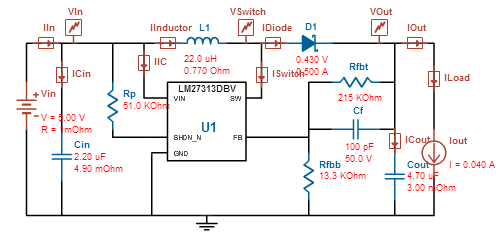
\includegraphics{21V_Schematic}
	      	\end{center}
	      	\caption{Schéma utilisé pour la simulation}
	      \end{figure}
	      	                  
	      Les valeurs retenues sont les suivantes :
	      	                  
	      \begin{center}
	      	\begin{tabular}{|c|c|}
	      		\hline
	      		Valeur d'inductance & Capacité de sortie \\
	      		\hline
	      		22 uH               & 4,7 uF              \\
	      		\hline
	      	\end{tabular}
	      \end{center}
	      	                  
	      En régime permanent, nous avons une tension de sortie qui varie très peu.
	      	                  
	      \begin{figure}[H]
	      	\begin{center}
	      		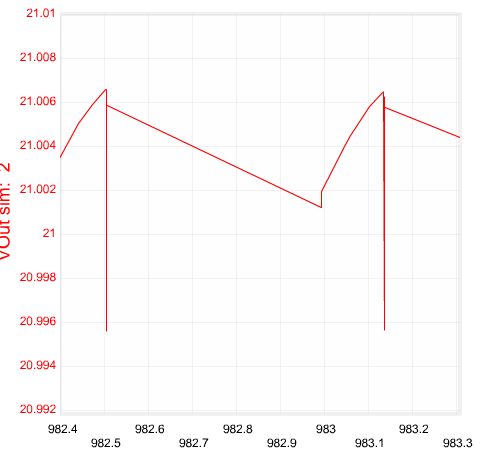
\includegraphics{21V_Steady_Vout}
	      	\end{center}
	      	\caption{Tension de sortie}
	      \end{figure}
	      	                  
	      La simulation estime le rendement à 70\% ce qui n'est pas particulièrement étonnant compte tenu du faible courant de charge.
          
	      Pour conclure sur les alimentations, on notera que les Buck et Boost choisi sont protégés en court-circuit puisqu'ils disposent d'un \angl{Thermal shutdown} arrêtant le découpage en cas de surchauffe des ICs.
	      Nous veillerons également à utiliser des condensateurs céramiques en entrée et en sortie avec un diélectrique X5R ou X7R pour la stabilité de leur capacité en température et leur \gls{ESR}/\gls{ESL} faible.
	      Ce dernier critère est particulièrement important, car un \gls{ESL} important viendrait déstabiliser la boucle de régulation déplaçant ses pôles.
	      	                  
	      Des LEDs ont été placées pour indiquer la présence des bonnes tensions.
	      On utilisera un transistor en saturé-bloqué pour la LED indiquant la présence du 21V pour éviter d'avoir une chute de tension trop importante au niveau de la résistance de limitation de courant de la LED.
	      Cet étage a été dimensionné en simulation avec LTSpice.
	      	                  
	\item \hyperlink{Schematic.3}{STM32F429ZI} :
	      le découplage du MCU est crucial pour son bon fonctionnement. 
	      Les capacités limitent la circulation de fortes variations des courants la carte. 
	      En effet, ce sont elles qui répondent aux fortes demandes de courant lors des commutations et ce sont elles qui mettent à la masse toutes les perturbations haute fréquence qui peuvent se retrouver sur le rail d'alimentation.
	      Elles servent également de réserve d'énergie locale en cas de microcoupures de l'alimentation. \\
	      La \angl{rule of thumb} impose 100 nF par pin d'alimentation + une plus grande capacité servant de réservoir d'énergie local. \\
	      Nous choisi d'utiliser un quartz pour générer l'horloge principale du MCU.
	      C'est un Quartz Crystal de 8 MHz que nous avons choisi.
	      Il permet d'avoir une horloge plus précise que l'horloge interne du MCU (± 50 ppm max.).\\
	      Par ailleurs il faudra faire attention à bien câbler les signaux sur les bonnes entrées.
	      Avec 144 broches, l'erreur est vite arrivée.\\
	      	                  
	\item \hyperlink{Schematic.4}{RAM} : de la même manière que pour le MCU, le découplage de la RAM est crucial pour son bon fonctionnement.
	      Nous avons appliqué les mêmes règles ici.\\
	      	                  
	\item \hyperlink{Schematic.5}{NOR} : de la même manière que pour le MCU, le découplage de la NOR est crucial pour son bon fonctionnement.\\
	      La principale difficulté de la NOR a déjà été mentionnée auparavant : le câblage du signal RY/BY\#.
	      En effet, ce signal indique au MCU la fin d'opérations longue telles que l'écrasement d'un secteur par exemple.
	      Le problème est que ce signal rentrait en conflit avec un des bits de données de l'écran LCD et la question que l'on s'est posée a été de savoir si on pouvait se passer de ce signal ou pas.
	      Après quelques recherches (l'information n'a pas été simple à trouver et à nécessitée la consultation des sources des pilotes logiciels), il s'est avéré que l'interface \gls{CFI} permet à un pilote générique d'interroger la mémoire NOR afin de récupérer les valeurs maximales des temporisations d'écrasement.
	      Ainsi ce signal n'est pas indispensable.
	      Nous l'avons quand même par précaution câblé sur une des entrées libres du MCU.\\
	      	                  
	\item \hyperlink{Schematic.6}{USB} : pour des raisons de sécurité et de conformité à la norme USB, nous avons choisi de rajouter un étage de protection sur les pistes VBUS de l'USB d'alimentation et de l'USB OTG.
	      Il s'agit du TPS2552DBVT de TI qui est un limiteur de courant commandable dont les caractéristiques principales sont les suivantes :
	      	                  
	      \begin{itemize}
	      	\item \angl{Up to \textbf{1.5 A} Maximum Load Current}
	      	\item \angl{Meets USB Current-Limiting Requirements}
	      	\item \angl{Adjustable Current Limit, 75 mA–1300 mA (typ)}
	      	\item \angl{\textbf{85-mΩ High-Side MOSFET}} : donc pertes en conduction faibles. 
	      	      Ce critère est extrêmement important si on veut optimiser la consommation énergétique de notre montage et diminuer la chute de tension aux bornes du MOSFET.
	      	      Rappelons que c'est le premier étage à l'entrée de notre carte.
	      	\item \angl{Reverse Input-Output Voltage Protection}
	      	\item \angl{Fast Overcurrent Response - 2-us (typ)}
	      	\item \angl{15 kV ESD Protection}
	      \end{itemize}
	      	                  
	      Ce circuit limite le courant en cas de court-circuit à une valeur maximale que l'on fixe de manière hardware et bloque le MOSFET pour couper le courant si la panne dure et que le circuit s'échauffe.
	      Il protège également en cas de surtension ou de \angl{reverse voltage} (tension de sortie > tension d'entrée) en bloquant le MOSFET.\\
	      Il servira donc, sur l'USB d'alimentation, à protéger l'alimentation sur laquelle la carte sera connectée en cas de court-circuit suite à une erreur de manipulation ou une panne de composant. \\
	      Et sur l'USB OTG, il protégera la carte si celle-ci est hôte (et donc délivre le 5V) en cas de défaillance du device qui est connecté (que ce soit un court-circuit ou une surtension) ou inversement protégera l'hôte sur lequel est connectée notre carte dans le cas où celle-ci est device. \\
	      Il est capable de signaler une défaillance au MCU avec le signal FAULT\#.\\
	      On peut également utiliser ces circuits comme interrupteurs commandables puisqu'ils disposent d'une broche EN\#.
	      On pourrait imaginer vouloir couper l'alimentation d'un périphérique USB par exemple ou redémarrer brutalement le MCU en envoyant un 0 sur l'EN\# du circuit en entrée de l'alimentation (le circuit redémarre tout seul parce qu'il y a une pull-down sur les EN\#)
	      	                  
	\item \hyperlink{Schematic.7}{Périphériques I/O} : le LCD a été relativement compliqué à câbler à cause d'une incompatibilité de notre MCU avec le protocole RGB888 qu'attend le driver de l'écran.
	      En effet, notre MCU avec le boîtier que nous avons choisi TQFP144 est capable de générer au plus du RGB666, malgré le fait que la datasheet mentionne affirme le contraire (comme quoi...).
	      La solution que nous avons choisi a donc été de relier ces bits de poids faibles à la masse.        
\end{itemize}
      
\subsubsection{Routage}       
\begin{itemize}
	\item Fabricant du \gls{PCB} : le ClubElek est sponsorisé par Cirly \autocite{Cirly} spécialiste lyonnais de la fabrication rapide de circuits imprimés prototypes et petites séries.
	      C'est en principe eux qui fabriqueront notre carte.
	      Un membre du binôme (Badr) est allé visiter leur usine située à Brignais, c'était une visite très enrichissante.
	      Il a pu découvrir le process de fabrication et discuter avec eux des éventuelles contraintes à garder en tête lors de la conception de \gls{PCB} 4 couches.
	          
	      \begin{figure}[H]
	      	\begin{center}
	      		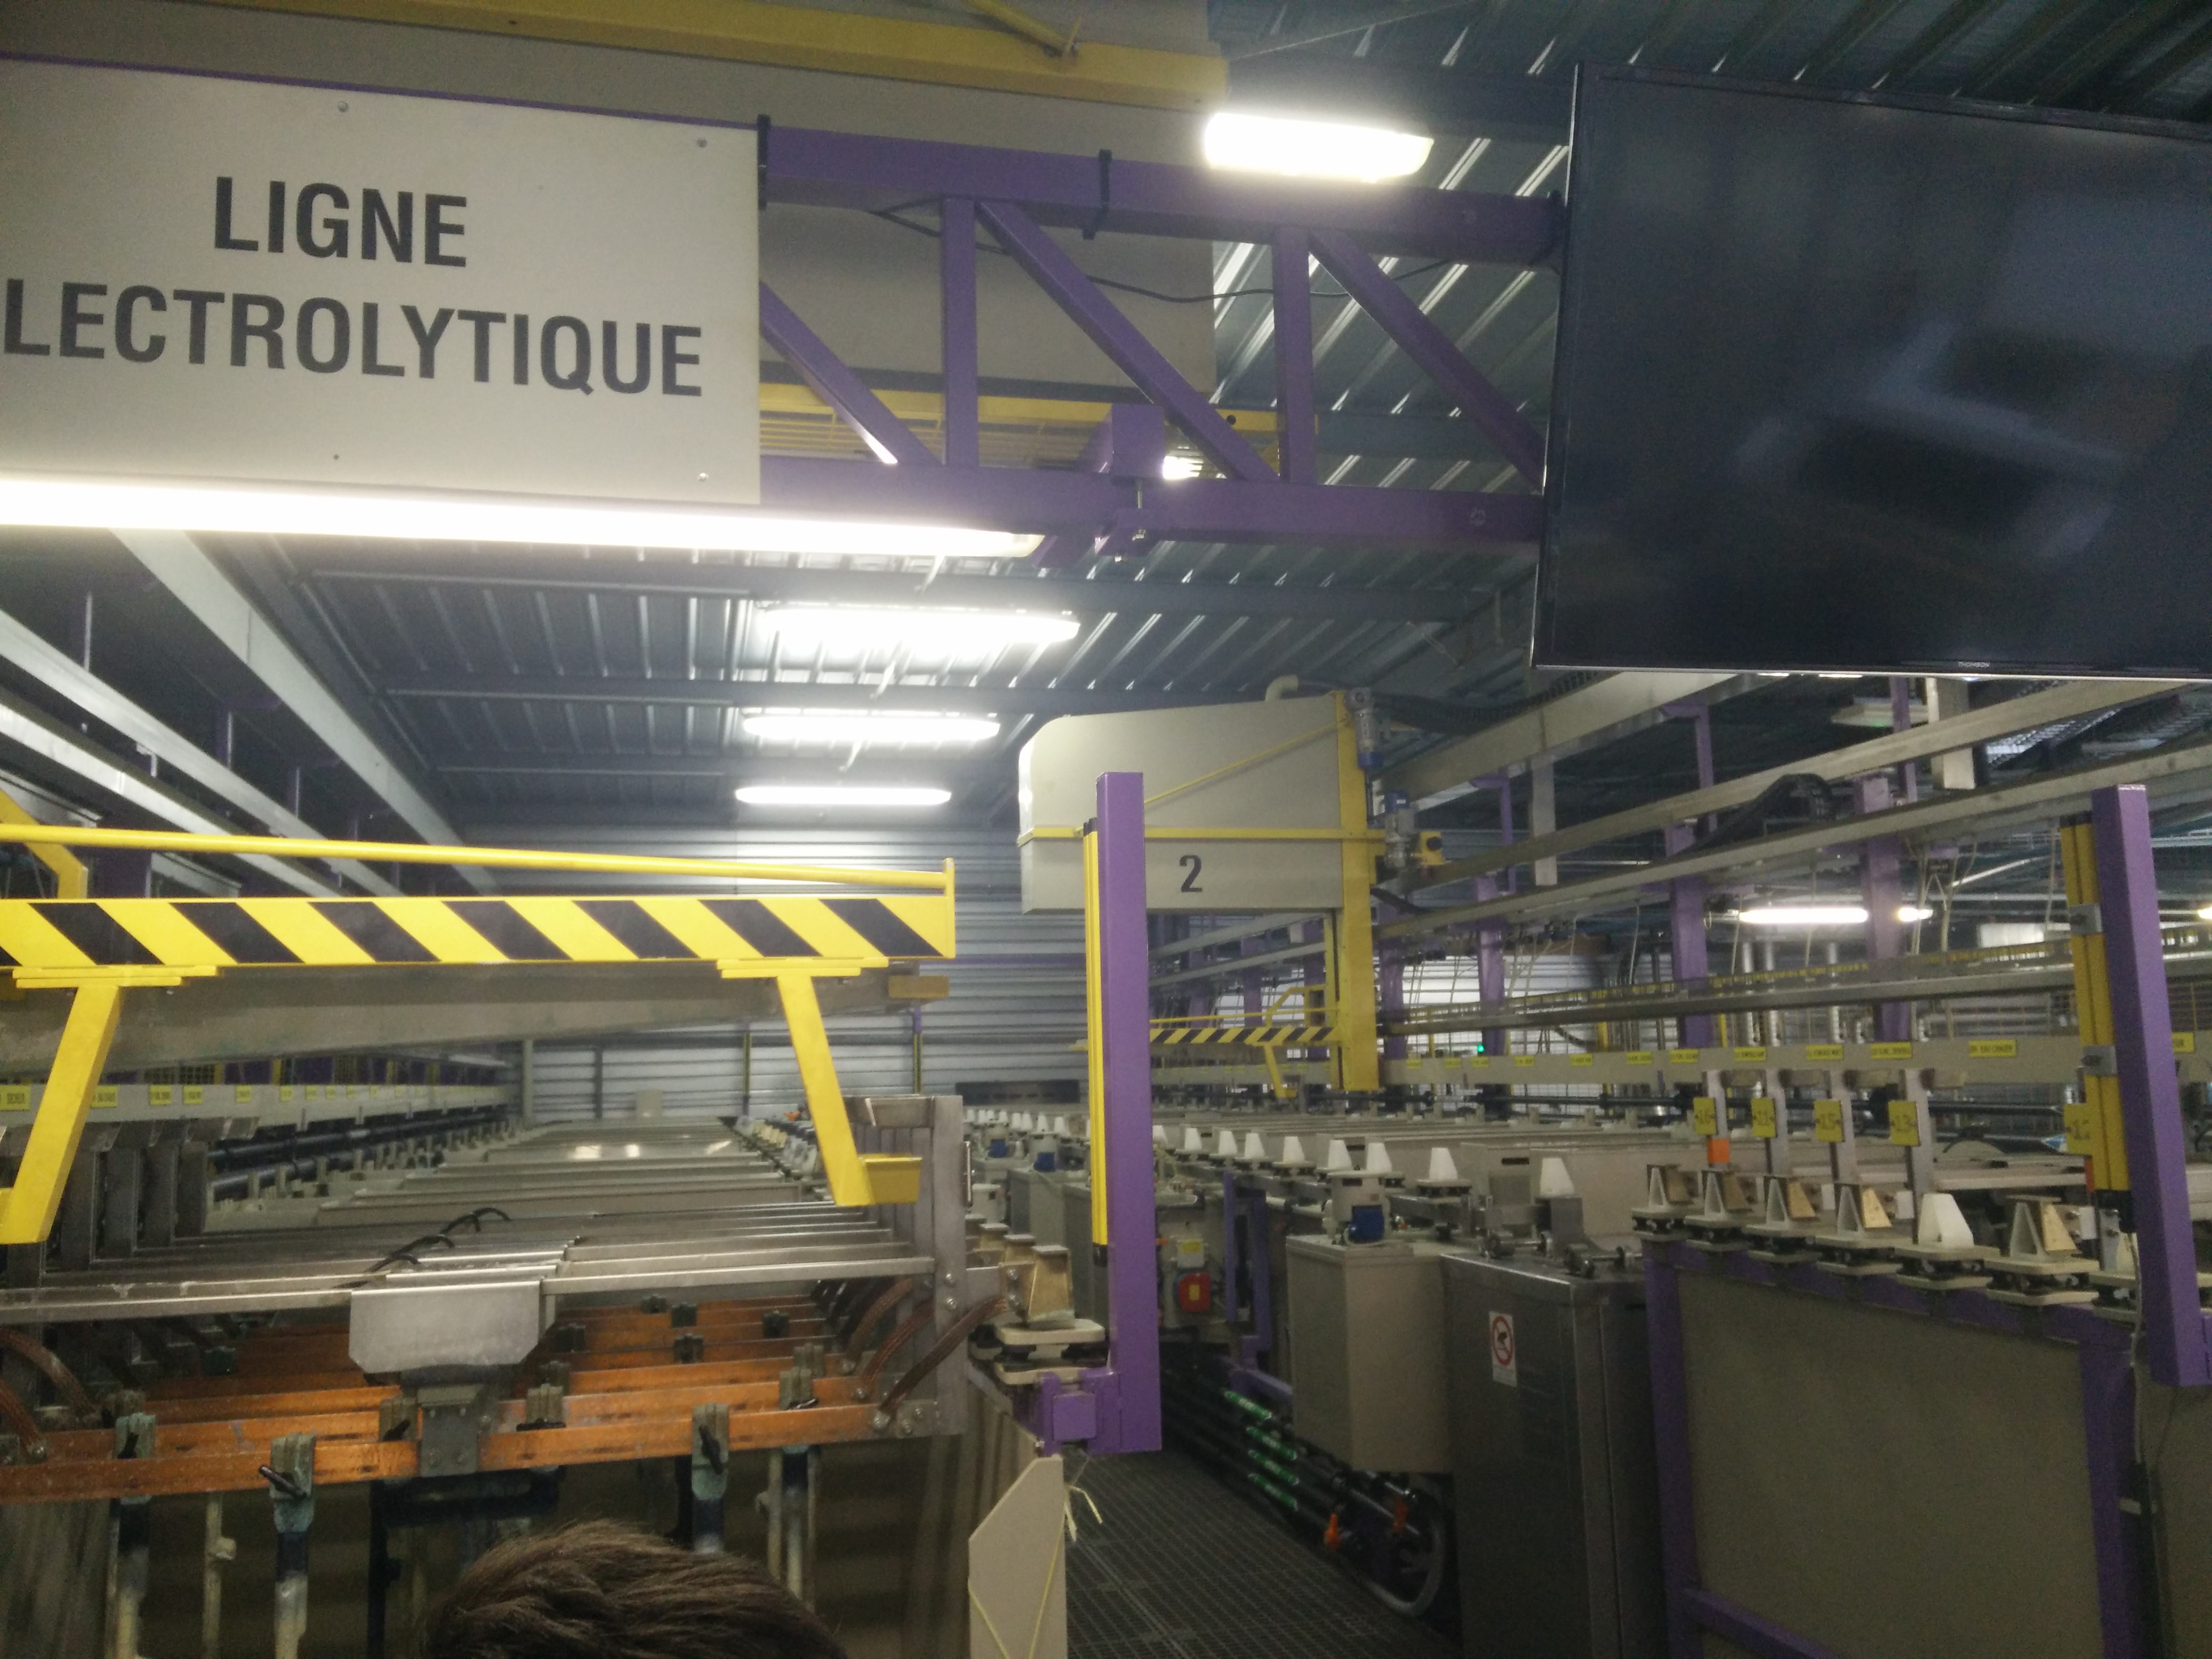
\includegraphics[scale = 0.1]{Cirly_usine}
	      	\end{center}
	      	\caption{Ligne d'électrolyse à l'usine de Cirly}
	      \end{figure}
	                
	\item Taille du \gls{PCB} : en vue d'une éventuelle intégration par la suite de cette carte dans une mécanique, nous choisisons de la faire la plus compacte possible. \\
	      Nous choisisons un \gls{PCB} rectangulaire de 70x43mm (70/43 = 1,62 ; tiens, c'est le chiffre d'or ?).
	      Plus sérieusement, ce \angl{template} s'appelle Sick of Beige \autocite{DPSOB}. C'est un format utilisé dans le monde des hobbyistes, il a été proposé par le blog Dangerous Prototypes pour uniformiser les \gls{PCB} faits dans le monde de l'OpenHardware. Dangerous Prototypes propose également des protections et supports pour ce format de \glspl{PCB}.
	          
	      \begin{figure}[H]
	      	\begin{center}
	      		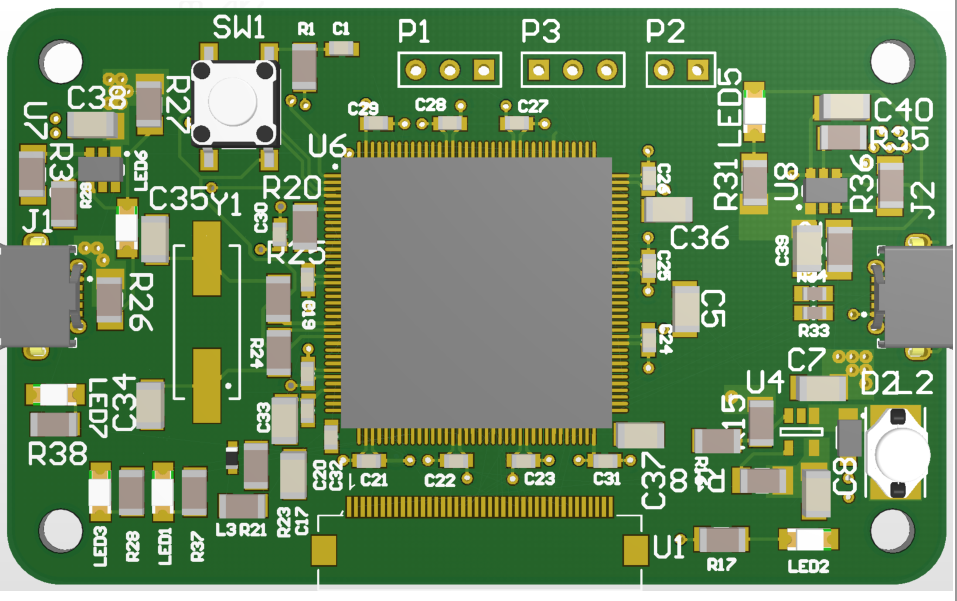
\includegraphics[scale = 0.55]{PCB_3D}
	      	\end{center}
	      	\caption{Vue 3D du PCB}
	      \end{figure}
	          
	\item \angl{Stack-up} : compte tenu de la taille du \gls{PCB} et du nombre de composants et signaux à router, on peut penser que la densité sera assez haute.
	      Nous choisisons donc d'utiliser 4 couches pour ce routage.
	      Le stack-up définit donc l'empilement de ces couches.
	      Il est important de bien définir son stack-up en prenant en compte : 
	      \begin{itemize}
	      	\item Le coût et les contraintes de fabrications : le coût augmenter (et de manière non linéaire!) avec le nombre de couches, les fabricants de \gls{PCB} proposent un certain nombre de stack-ups 'standard' même si les matériaux (épaisseurs, constantes diélectriques principalement) varient d'un fabricant à l'autre. 
	      	      Généralement, il est financièrement plus intéressant d'adapter son stack-up à ce que propose le fabricant.
	      	\item Les contraintes CEM : un bon stack-up optimise la CEM et diminue la sensibilité des circuits aux parasites électromagnétiques.
	      \end{itemize}
	      N'ayant pas de contraintes CEM ni de contraintes de sensibilité électromagnétique, nous tiendrons compte seulement des deux premiers critères. \\
	      Nous avons demandé un dossier technique à Cirly et le stack-up retenu est finalement le suivant :
	          
	      \begin{figure}[H]
	      	\begin{center}
	      		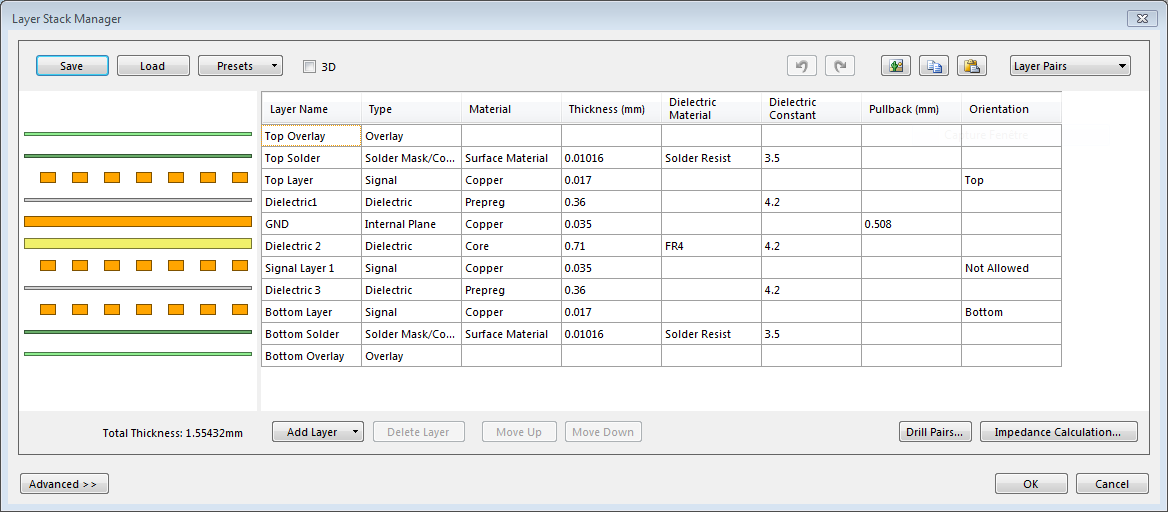
\includegraphics[scale = 0.45]{Stack-up}
	      	\end{center}
	      	\caption{Stack-up utilisé pour le PCB}
	      \end{figure}
	                
	      On peut voir que nous avons renseigné l'ordre d'empilement des différentes couches, les types de matériaux utilisés, leurs épaisseurs ainsi que leurs constantes diélectriques (utilisées pour calculer les impédances des pistes). 
	      	
	\item Placement et routage :
	      Un bon routage réduit la majorité des problèmes (et c'est d’autant plus intéressant qu’il n’a aucune incidence sur la BOM, il n’y a pas de compromis coût/routage à faire). 
	      Quelques principes de base que nous essayions de respecter au maximum lors de ce routage (et tout le temps de manière générale) :
	      \begin{itemize}
	      	\item Sur les cartes mixtes (analogique/numérique) : un seul plan de masse avec zonage des parties mixtes.
	      	      Cela sert à garder une relative maîtrise de la circulation des courants sur la carte.
	      	\item Tracer des pistes formant les boucles les plus courtes possible.
	      	\item Les capacités de découplage doivent être placées au plus près des composants. 
	      	      Il faut éviter les vias entre les capacités de découplage et les IC car les vias sont fortement inductives (plus inductives qu’une piste).
	      	\item Faire attention aux diaphonies par couplage capacitif ou inductif. Une perturbation sur un conducteur va injecter un signal perturbateur sur le conducteur voisin. Ce couplage peut avoir deux origines :
	      	      \begin{enumerate}
	      	      	\item Lorsqu’un conducteur est soumis à une d.d.p., la capacité mutuelle (notée \(C_m\)) injecte un courant perturbateur sur le conducteur voisin. 
	      	      	      C’est la diaphonie capacitive.
	      	      	\item Lorsqu’un courant circule dans un conducteur, il génère un champ magnétique qui se couple dans la boucle formée par le conducteur voisin par rapport à la masse. 
	      	      	      C'est la diaphonie inductive.
	      	      \end{enumerate}
	      	\item L'égalisation de la longueur des pistes sur les bus de données et d'adresses des mémoires est conseillée pour avoir des temps de propagations égaux.
	      	\item L'égalisation de la longueur des pistes et la symétrie des pistes de bus différentiels (le D+ et D- du bus USB par ex.) est conseillée.
	      	\item L’utilisation d’un plan de masse permet de réduire de façon importante la diaphonie entre pistes lorsque la distance entre pistes est supérieure à la hauteur par rapport au plan de masse. 
	      	      La présence d’un plan de masse réduit la diaphonie de façon très significative.
	      	      C’est pour cela qu’il vaut mieux placer, dès que possible, des plans de masse dans le stack-up pour diminuer la diaphonie entre pistes sensibles (horloges, bus haute vitesse, pistes d’alimentations à découpage, etc.).
	      	\item Réduire les problèmes de CEM consiste avant tout à améliorer l’équipotentialité des systèmes en HF.
	      	\item Un plan de masse ne doit pas être fendu.
	      	      Un plan de masse fendu voit son impédance fortement augmenter en HF. 
	      	      Il a une impédance très faible tant qu’il reste homogène.
	      	\item Un anneau de garde en bord de carte relié à la masse est une bonne pratique pour encaisser les ESD et augmenter l’équipotentialité des masses.
	      \end{itemize}
	          
	      Il faut être attentif, minutieux, cohérent et logique dans son routage en respectant les règles de base citées ci-dessus et toutes autres règles que l’on s’impose.
	      Parmi les quelques erreurs récurrentes que nous essayions d'éviter :
	      \begin{itemize}
	      	\item Changement des largeurs de pistes en cours de route (éviter de former des goulots d'étranglement)
	      	\item Angles droits sur les pistes
	      	\item Pistes sensibles placées en dessous d’inductances
	      	\item Pistes formant des boucles très larges
	      	\item Plans de masse fendus
	      	\item Placements de capacités de découplage non optimisé
	      \end{itemize}
	          
              
	      \begin{figure}[H]
	      	\begin{center}
	      		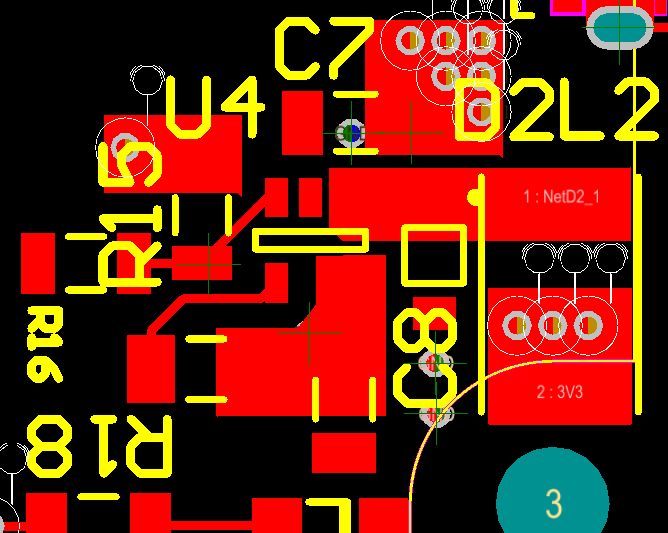
\includegraphics[scale = 0.8]{Exemple_Routage_Buck}
	      	\end{center}
	      	\caption{Exemple de placement et routage du Buck}
	      \end{figure}
	          
	      Nous avons essayé de garder la piste entre D2 et L2 la plus courte possible. Vu que ce sont des composants qui vont 'voir' le découpage, les inductances parasites des pistes risquent d'augmenter les résonances et les bruits. 
	      Nous avons également essayé de rapprocher R15, R16 et la broche FB dans le but d'éviter d'avoir du bruit qui s'ajoute à au signal de \angl{feedback} et qui, de fait, perturberait la régulation.
	      Nous avons également augmenté le nombre de vias connectant le plan de masse du Buck au plan de masse global pour augmenter l'équipotentialité des masses et diminuer l'impédance de celle-ci.
	      Cela diminue les pertes, mais surtout réduit le bruit rayonné et conduit.
	          
\end{itemize}

\subsubsection{Procédure de test et board bring-up}       
	Afin de s'assurer du bon fonctionnement de la carte, il est nécessaire de la tester une fois soudée.
    
    Le premier test à effectuer est la validité des soudures, car des courts-circuits sont assez susceptibles d'être présents à cause du boîtier du microcontrôleur.

	Une fois les soudures validée, il faut tester le bon fonctionnement des Buck et Boost en s'assurant qu'ils délivrent les bonnes tension.
    
    Enfin, un test de programmation de la mémoire interne du microcontrôleur permettra d'envoyer un programme de test (U-Boot) que l'on exécutera et qui permettra de valider la bonne exécution du code et l'usage de l'UART.

\section{Software}
La partie logicielle de ce projet consiste en la création d'un firmware basé sur un système GNU/Linux.
Elle nécessite donc l'utilisation d'un certain nombre de composants logiciels dont il faut récupérer les sources, les paramétrer et les compiler.
Cette opération peut prendre un certain temps, car il faut s'assurer de la compatibilité de différentes versions qui n'ont pas été nécessairement testées ensemble.
Il est donc indispensable d'être aux faits des types de changement que chaque brique peut apporter à son interface afin de savoir où peuvent se situer les problèmes potentiels.
Un exemple évident de ce problème serait un programme utilisant un appel système qui ne serait pas implémenté dans la version du noyau utilisée, ou un programme nécessitant la glibc alors qu'une autre libc est utilisée.
La figure \ref{libc} illustre la position occupée par la libc dans un système GNU/Linux.
\begin{figure}[H]
	\begin{center}
		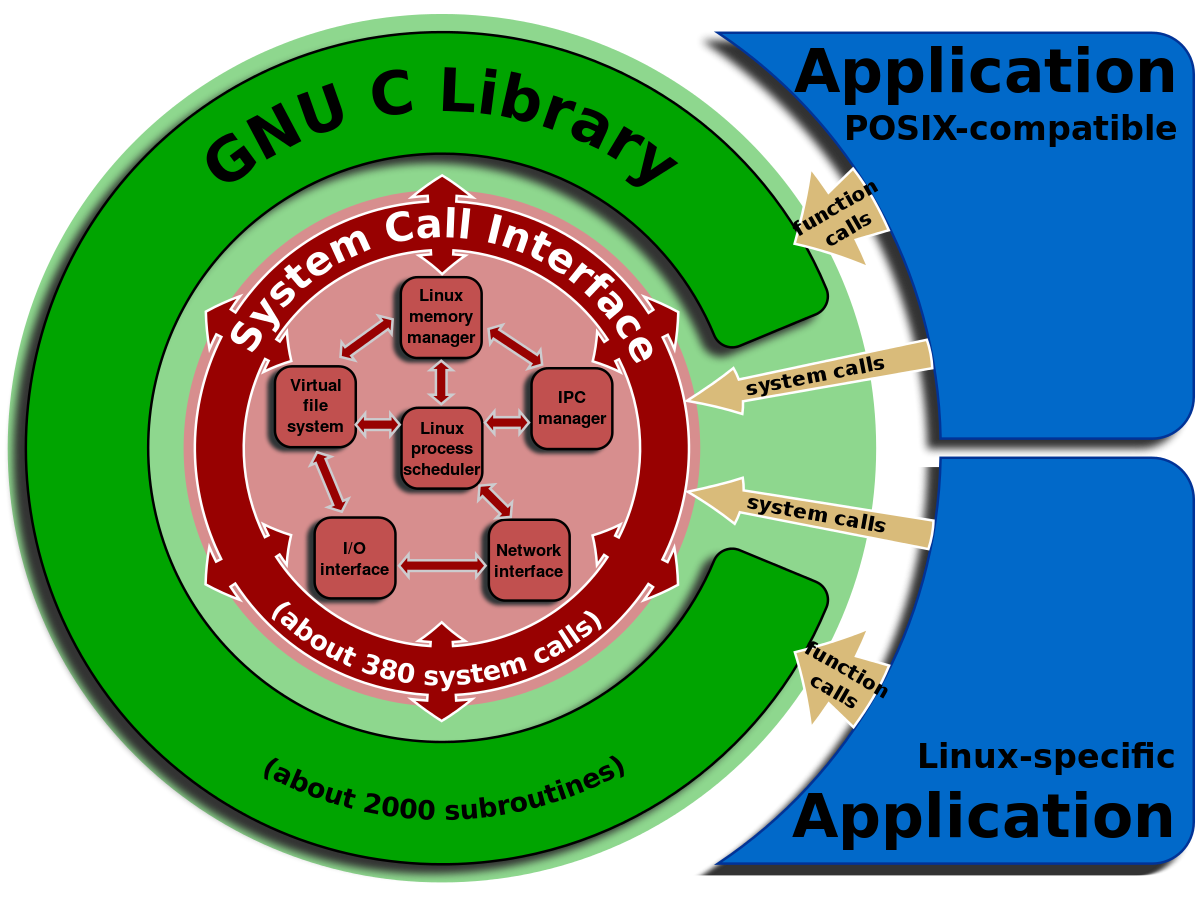
\includegraphics[scale = 0.3]{Linux_kernel_System_Call_Interface_and_glibc}
	\end{center}
	\caption{Place de la libc dans un système GNU/Linux}
	\source{\url{http://commons.wikimedia.org/wiki/File:Linux_kernel_System_Call_Interface_and_glibc.svg}}
	\label{libc}
\end{figure}
    
On a donc les mêmes problématiques qu'un \angl{packageur} d'une distribution dont le rôle est de compiler les différents logiciels en s'assurant que ses dépendances sont satisfaites dans les bonnes versions et en appliquant des patchs si nécessaire.
    
La figure \ref{LinuxAPIStability} illustre la problématique de stabilité des interfaces telle qu'on la trouve dans le logiciel libre, du fait de l'indépendance des projets et de l'infinité de configurations et variations possibles dans les sources modifiées.
\begin{figure}[H]
	\begin{center}
		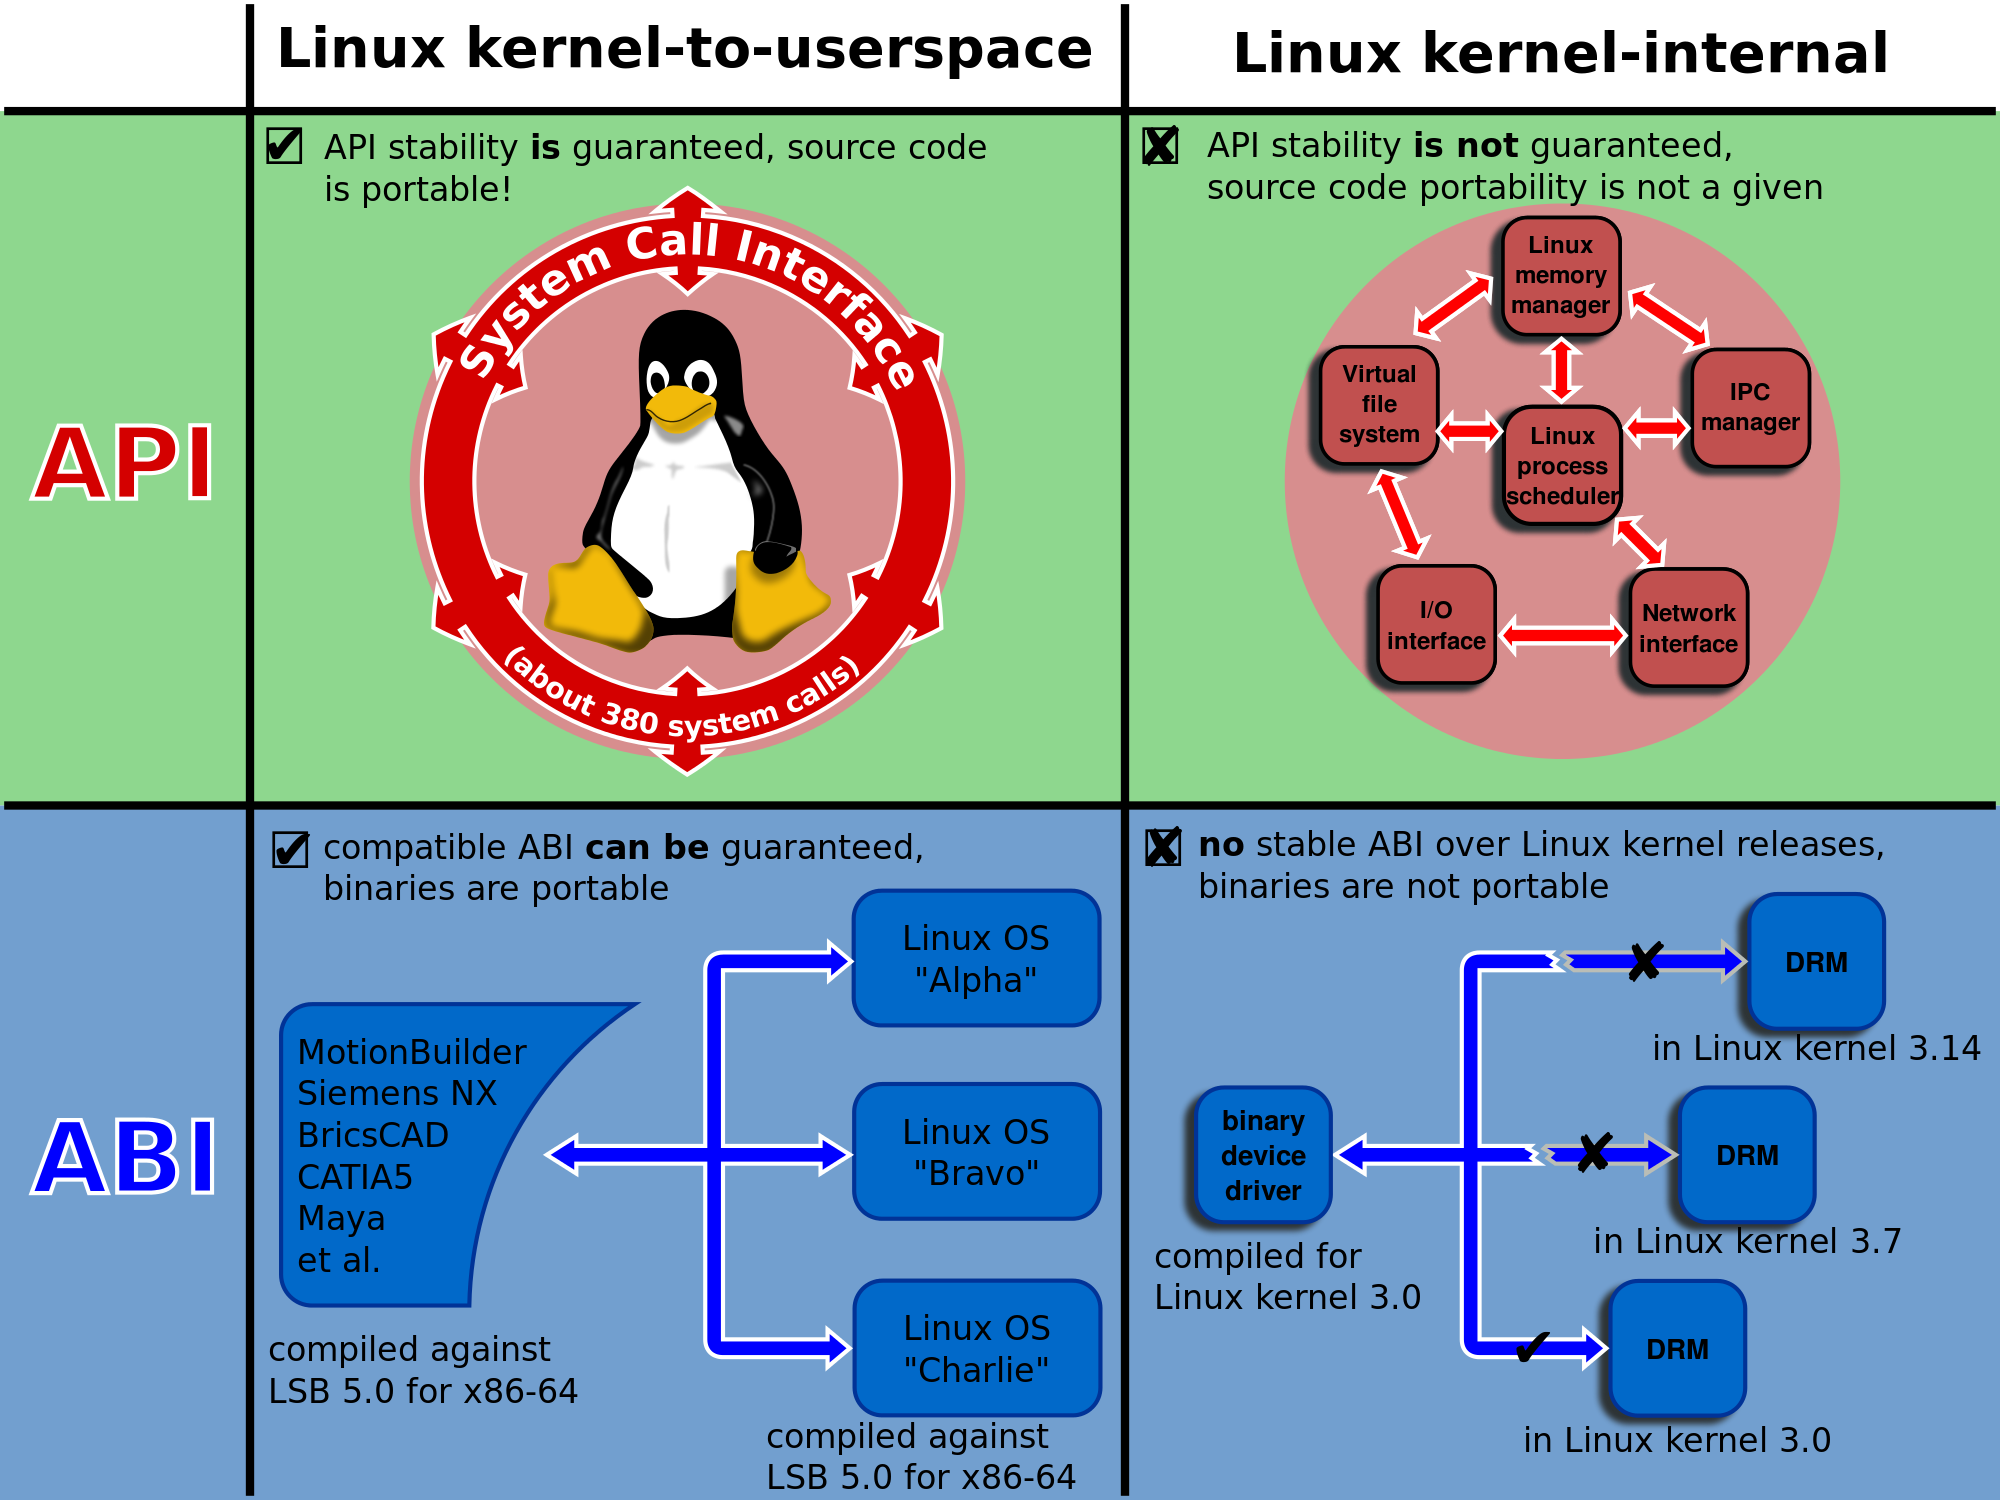
\includegraphics[scale = 0.2]{Linux_kernel_interfaces}
	\end{center}
	\caption{Stabilité des interfaces du noyau Linux}
	\source{\url{http://commons.wikimedia.org/wiki/File:Linux_kernel_interfaces.svg}}
	\label{LinuxAPIStability}
\end{figure}
    
\subsection{Architecture générale}
Étant données les contraintes de place dans la mémoire de la carte de développement utilisée pour le prototypage logiciel (2Mo de Flash interne), ainsi que dans la carte finale, il est nécessaire de construire le système le plus minimal possible.
Ce n'est donc pas une distribution GNU/Linux tel que Debian ou même Ångström qui est utilisé mais un ensemble de composant logiciel choisi, configurés et compilés afin de constituer un système de fichier racine permettant un démarrage et une exploitation basique de la carte.

\subsubsection{Noyau}
Le noyau utilisé est le noyau uClinux, qui est une variante du noyau Linux pouvant s'exécuter sur des processeurs ne possédant pas de \gls{MMU} \autocite{uClinuxLinuxDiff}.
Un certain nombre de fonctionnalités reliées à la présence de mémoire virtuelle sont absentes, tels qu'un comportement différent pour certaines options de \texttt{mmap} ou encore l'appel système \texttt{fork} (seul \texttt{vfork} est implémenté, car sans \gls{MMU}, il est impossible d'implémenter le comportement copy-on-write lors de la création du nouvel espace d'adressage pour le processus).
La stabilité du système est aussi plus faible, car un processus utilisateur peut corrompre la mémoire de n'importe quel programme, même le noyau, à moins que la \gls{MPU} ne soit utilisée.
				
\begin{figure}[H]
	\begin{center}
		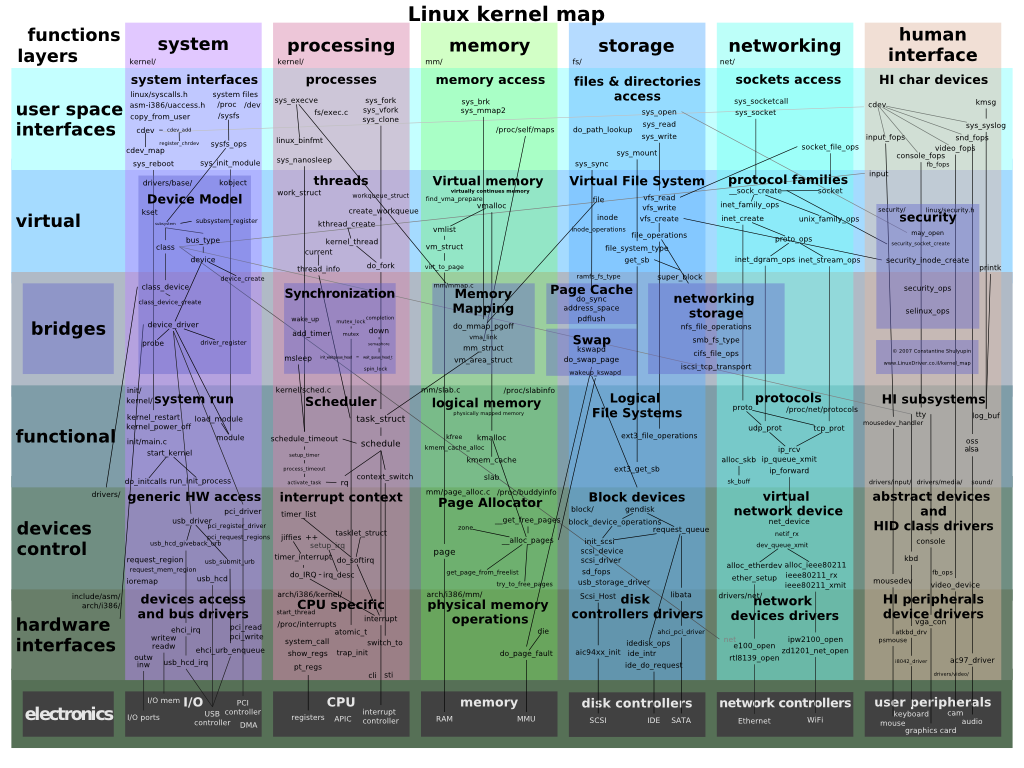
\includegraphics[scale = 0.4]{Linux_kernel_map}
	\end{center}
	\caption{Carte du noyau Linux}
	\source{\url{http://www.makelinux.net/kernel_map/}}
\end{figure}

\subsubsection{Bootloader}
Le bootloader U-Boot est le logiciel permettant d'amorcer l'exécution du noyau uClinux.
Il permet également de reprogrammer la mémoire flash et propose une interface basique en ligne de commande accessible sur une UART.
Il réalise différentes tâches d'initialisation telles que celles des mémoires externes (initialisation du \gls{FMC}).

\subsubsection{Espace utilisateur}
La racine est presque exclusivement constituée du binaire de BusyBox \autocite{BusyBox}, qui est un programme implémentant les commandes les plus basiques ainsi qu'un shell ash \autocite{Ash}.
Quelques scripts d'initialisations sont également présents dans /etc, ainsi que les fichiers de périphériques de /dev (le système de fichier ROMFS \autocite{ROMFS} étant en lecture seule, on ne peut pas utiliser directement d'outils tels que mdev ou udev pour peupler dynamiquement /dev/).

\subsubsection{Système de fichier ROMFS}
Ce système de fichier basique en lecture seule permet d'utiliser au mieux la mémoire Flash disponible.
Il n'utilise presque pas d'espace pour la gestion des fichiers, mais il est uniquement disponible en lecture seule.
Il faut utiliser l'outil genromfs \autocite{ROMFS} afin de générer une image ROMFS.
Cet outil transforme une arborescence en fichier prêt à être écrit en mémoire.
Un avantage de ce système de fichier outre sa compacité est son support de l'\gls{XIP}.
Il est ainsi possible d'exécuter le code directement depuis la Flash, sans avoir à le copier en RAM, ce qui fait économiser autant de mémoire vive.
        
\subsection{Solutions existantes}
Des systèmes utilisables sur la carte d'évaluation STM32F429 Discovery sont mis à disposition sur des dépôts Git sur GitHub.
Le principal est celui de la société Emcraft \autocite{Emcraft}:~\url{https://github.com/EmcraftSystems/linux-emcraft.git}, l'autre étant celui de l'utilisateur Robutest:~\url{https://github.com/robutest/uclinux.git}.
Le dépôt de Robutest contient un système totalement prêt à l'emploi avec des Makefile pour le construire (bootloader, noyau, espace utilisateur), mais le noyau n'est pas le plus récent et n'inclut pas le pilote pour l'\gls{IP} USB Synopsys utilisé dans le STM32F429.
Le dépôt d'Emcraft contient uniquement un noyau un peu plus récent, avec le pilote, mais le noyau n'est pas forcément configuré correctement pour la carte de développement.
        
Une fusion des deux a été effectuée, en utilisant le noyau d'Emcraft plus récent et la configuration ainsi que le reste du système proposé par Robutest.
Cette phase de portage de la configuration n'est pas aussi aisée qu'elle parait, car des divergences existent entre les deux noyaux, et certaines options ont été ajoutées ou retirées.
Ainsi, il a également été nécessaire d'importer les modifications apportées à certains fichiers sources du noyau de Robutest qui n'ont pas été contribuées dans le noyau d'Emcraft et de résoudre divers problèmes de compilation.
Un \angl{build system} basé sur CMake a aussi été réécrit en reproduisant les fonctionnalités proposées par le dépôt de Robutest, pour améliorer la gestion des dépendances entre les composants et la facilité de développement d'une application indépendante.
On peut maintenant inclure un programme et l'installer dans l'arborescence générée pour la racine avec un simple fichier CMakeLists.txt classique de quelques lignes.

\subsection{Outils de développement}
Les outils de développement utilisés pour mener ce projet sont le compilateur GCC porté pour ARM Cortex-M, version 2010q1.
Cette version de GCC semble correctement compiler le noyau uClinux, ce qui est cohérent avec leurs dates de sortie proche.
Une archive du compilateur déjà compilé est disponible à cette adresse:~\url{https://sourcery.mentor.com/public/gnu_toolchain/arm-none-linux-gnueabi/\\arm-2010q1-202-arm-none-linux-gnueabi-i686-pc-linux-gnu.tar.bz2}.
Ce portage de GCC génère des fichiers ELF \autocite{ELF}, qui sont ensuite convertis au format BFLT \autocite{BFLT} qui est plus simple et autorise le \gls{XIP} permettant d'exécuter un programme directement depuis la mémoire flash NOR sans le copier en RAM.
Il est également fourni avec une version précompilée de la uClibc \autocite{uClibc} avec laquelle il link les programmes par défaut.
        
Un débogueur GDB est aussi fourni.
Celui-ci est un client se connectant à un serveur GDB, qui est en l'occurrence OpenOCD \autocite{OpenOCD}.
Il gère la communication avec la sonde \gls{SWD} ST-LINK/V2 embarquée sur la carte de développement STM32F429 Discovery.
        
Make est utilisé dans les \angl{build system} de Linux, BusyBox et U-Boot.
Il est invoqué par la CMake pour compiler ces programmes qui n'utilisent pas CMake pour leur \angl{build system}.
        
CMake est utilisé pour orchestrer la compilation des différents composants.
        
Enfin, la carte de développement STMicroelectronics STM32F429 Discovery a été utilisée afin de travailler sur la partie logicielle avant que notre carte soit prête physiquement.
        
Afin de gérer les sources de la partie logicielle du projet, un dépôt Git a été créée grâce au compte offert par Assembla \autocite{Assembla} .
        
Les documents \LaTeX{} des rapports ont été rédigés sur la plate-forme collaborative Overleaf \autocite{Overleaf} qui dispose d'une interface web collaborative proche de Google Drive (édition simultanée par plusieurs utilisateurs), en éliminant le besoin d'une installation locale de \LaTeX{} (Overleaf est basé sur Texlive).
Une fonctionnalité intéressante d'Overleaf est qu'un document peut être accédé comme un dépôt Git, permettant une synchronisation dans les deux sens.
Ceci permet de travailler hors ligne, et également de faire une sauvegarde à jour et de voir facilement les modifications apportées au cours du temps par les différents utilisateurs.        	

\subsection{Construction du firmware}
L'image du firmware prête à être écrite en RAM est donc produite en plusieurs étapes orchestrées avec CMake.
        
D'abord, les \angl{build system} basés sur des Makefile de uClinux, U-Boot et BusyBox sont appelés par CMake.
Ensuite, les programmes de l'utilisateur sont compilés avec CMake.
Une phase d'installation permet de peupler un dossier qui sera la racine du système uClinux.
Enfin, cette racine est transformée en image ROMFS grâce à genromfs, et on peut utiliser OpenOCD pour flasher le bootloader U-Boot, puis le noyau uClinux, puis l'image ROMFS dans la mémoire flash.

Pour que ces étapes produisent un système fonctionnel, il est impératif que U-Boot soit flashé à une adresse pour laquelle il a été construit, de même que le noyau uClinux.
Il faut également que l'image ROMFS soit écrite à l'adresse à laquelle le pilote MTD \autocite{MTD} de Linux s'attend à le trouver.


\subsubsection{Paramétrage du noyau uClinux}
Le noyau uClinux utilisé étant la fusion du noyau de Robutest (GitHub) et d'Emcraft (\angl{upstream} de Robutest, noyau plus récent), il a fallu adapter les options de configuration et porter les modifications de Robutest qui n'ont pas été remontées à Emcraft.
De plus, Robutest a configuré son noyau pour qu'il s'exécute correctement sur la carte d'évaluation STM32F429 Discovery, ce qui n'est pas le cas du noyau d'Emcraft.

Quelques options de configurations permettent de choisir l'adresse à laquelle le noyau s'exécutera pour que l'édition des liens se fasse correctement (le \angl{linker script} tient compte de cette adresse).
Cette adresse doit également être connue de U-Boot afin qu'il puisse trouver le noyau et le lancer.
D'autres options permettent d'activer les MTD \autocite{MTD} qui sont l'abstraction fournie par le noyau Linux pour les mémoires flash accessibles directement (et non pas via une \gls{FTL}).

\subsubsection{Paramétrage du bootloader U-Boot}
Le paramétrage de U-Boot est assez direct.
L'activation de trop d'options augmente sa taille, mais elles peuvent se révéler pratiques en phase de développement (shell permettant de reprogrammer la mémoire par exemple).
Il faut indiquer les options à passer au noyau lors de l'amorçage, ainsi que son adresse en mémoire.

\subsubsection{Paramétrage de BusyBox}
La dernière version stable de BusyBox (1.23.2) est utilisable.
Il faut choisir les options à activer, plus il y en a, plus le binaire final est gros, ce qui peut poser problème sur la carte de développement STM32F429 Discovery qui ne possède seulement que 2Mo de Flash interne.

\subsubsection{Utilisation des différentes mémoires}
L'utilisation des mémoires suivantes permet d'exploiter au mieux les ressources de la carte~:
\begin{itemize}
	\item Flash interne (2Mo): Bootloader U-Boot (\~70Ko) + Noyau uClinux (\~700Ko)
	\item RAM interne (256Ko): Pile du noyau (4Ko)
	\item NOR externe (32Mo): Userspace (XIP)
	\item SDRAM externe (16Mo): Données des programmes externes et du noyau
\end{itemize}
La raison est la suivante~: la mémoire flash interne est accessible en un cycle, alors que la NOR externe est beaucoup plus longue à être lue.
Le contrôleur des mémoires externes \gls{FMC} du STM32F429 ne peut en outre servir qu'un accès à la fois.
Il est donc impossible d'accéder à la SDRAM en même temps qu'à la NOR, contrairement aux RAM et Flash interne d'après l'agencement de la matrice du bus \gls{AHB} interne du microcontrôleur \autocite{STM:ReferenceManual}.
Le composant le plus critique en terme de performance étant le noyau, c'est celui-ci qui est mis en flash interne, et sa pile en RAM interne (sa faible taille est idéale, et son accès sera rapide).
Ce changement est encore à valider, car il n'est pas l'objet d'une option de configuration, et a peut-être des répercussions non triviales sur d'autres parties du code.
Le bootloader réside forcément en Flash interne, car il doit s'exécuter avant l'initialisation du \gls{FMC}.
Enfin, les programmes non critiques sont placés en mémoire NOR externe, et leurs données en SDRAM externe pour des raisons d'espace mémoire.


\subsection{Validation du hardware}
La validation de la carte peut être réalisée à partir du bootloader U-Boot ainsi que d'OpenOCD.
Une connexion d'OpenOCD et une programmation de la flash interne indiquent un bon fonctionnement du microcontrôleur, et la bonne exécution de U-Boot permet de valider une application \angl{bare-metal} raisonnablement simple.
        
Par ailleurs, il est nécessaire de tester la mémoire SDRAM et NOR afin de vérifier que les informations de timing sont correctement renseignées et que la SDRAM fonctionne de manière prédictible et sans erreur. 
U-Boot dispose d'une commande \texttt{mtest} permettant de tester des plages de mémoires.
De la même manière, OpenOCD peut être scripté en Jim TCL afin de réaliser un test de lecture écriture de la mémoire.
	
\subsection{Prévision des performances}
Les performances de calcul de cette carte seront selon toute vraisemblance relativement faibles par rapport à une carte intégrant un processeur avec des caches.
On a en effet un goulet d'étranglement majeur au niveau du \gls{FMC} qui est un point de passage des données de la NOR et de la SDRAM externes.
De plus, la fréquence maximale à laquelle le \gls{FMC} peut faire fonctionner la SDRAM externe est $HCLK/2$, avec $HCLK$ l'horloge du bus \gls{AHB} interne auquel est lié le \gls{FMC} et qui est aussi l'horloge du cœur \autocite{STM:ReferenceManual}.
Avec une fréquence maximale de 180 MHz pour $HCLK$, le transfert du code et des données vers le cœurs diviseront probablement par 7 ou 8 la vitesse d'exécution par rapport à l'usage de la RAM et Flash interne.
        
Cependant, l'expérience de la carte de développement a prouvé que malgré ces chiffres relativement bas, il est tout à fait possible d'avoir un système réactif et sans lenteurs pour un usage de base.
        
Une amélioration possible serait d'utiliser les nouveaux ARM Cortex M7 qui implantent des mémoires cache dans le but de mieux gérer ce type d'architecture logicielle.


\sectionsansnumero{Conclusion}
Ce projet nous a permis de nous familiariser avec un certain nombre de composants tels que les mémoires NOR et SDRAM ainsi que les critères de choix qui leur sont associés.
Sur le plan matériel, l'intégration de tous les composants nécessaires sur une carte de petite dimension a été un défi et a été l'occasion d'apprendre et de se perfectionner dans l'utilisation d'Altium Designer.
Sur le plan logiciel, il a été l'occasion de se pencher sur les composants fondamentaux d'une distribution GNU/Linux ainsi que leur rôle exact et sur la mise en place des outils de développement associés.
Il a de plus mis en lumière l'interdépendance entre le logiciel et le matériel, en travaillant en équipe dont un membre est plus orienté sur l'aspect matériel et l'autre sur l'aspect logiciel.
Cette diversité de profil s'est révélée efficace et a permis d'avancer ce projet aux multiples facettes.

Nous n'avons pas atteint nos objectifs dans les temps impartis (arriver à démarrer Linux sur notre \gls{PCB}) parce que nous nous sommes heurtés à des problématiques auxquelles nous ne pensions pas, mais également parce que nous avons voulu faire les choses proprement et approfondir notre compréhension des concepts et phénomènes en jeu.
Nous regrettons que ce semestre de 4GE soit aussi dense et que le temps dédié au PRT soit limité par tout le reste.
Ce projet sera néanmoins poursuivi par la suite (juste après les partiels) dans le cadre d'un projet personnel.

\newpage{}
\sectionsansnumero{Annexe 1~: Schémas électriques de la carte}
\label{sec:AnnexeSchematic}

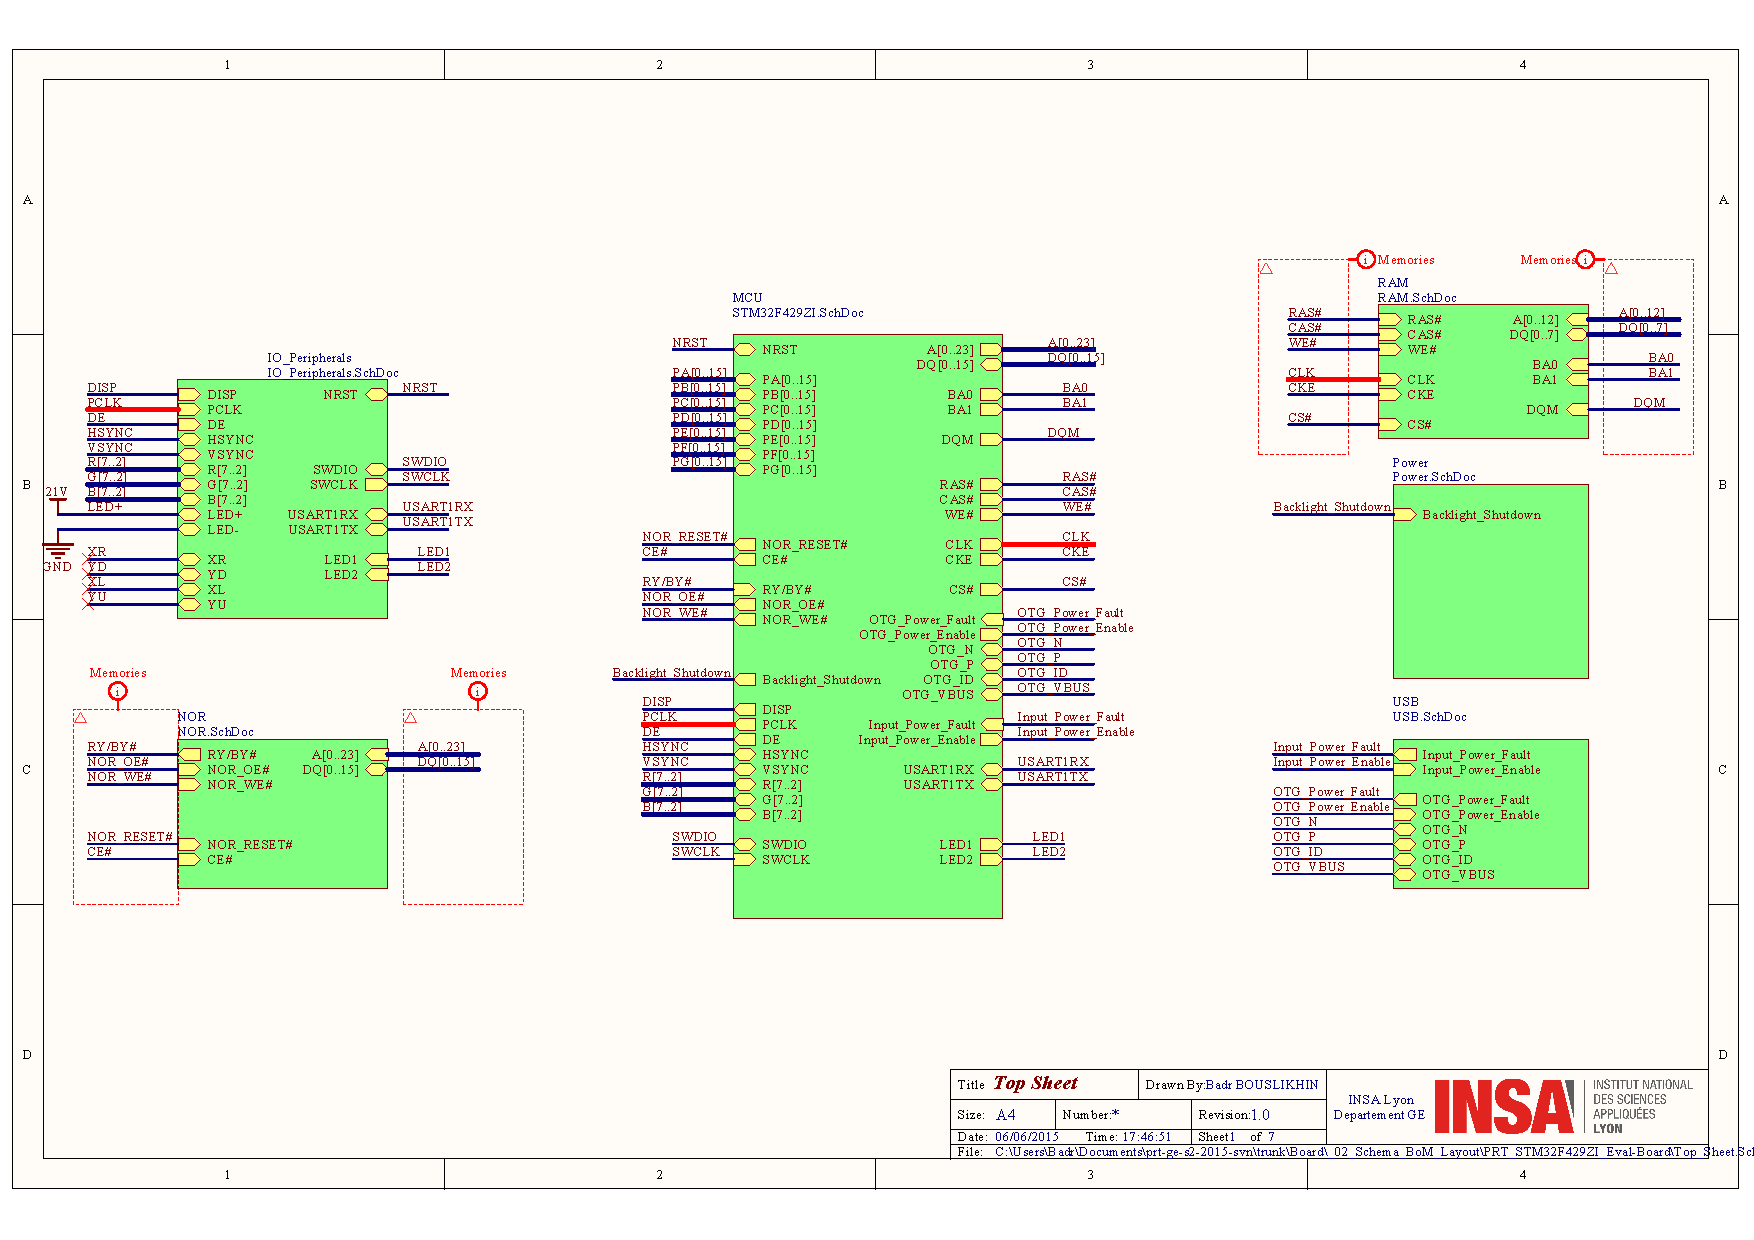
\includepdf[pages={1-}, link, linkname=Schematic, landscape=true]{PDF/PRT_STM32F429ZI_Eval-Board.pdf}

\newpage{}
\sectionsansnumero{Annexe 2~: Bill Of Material de la carte}
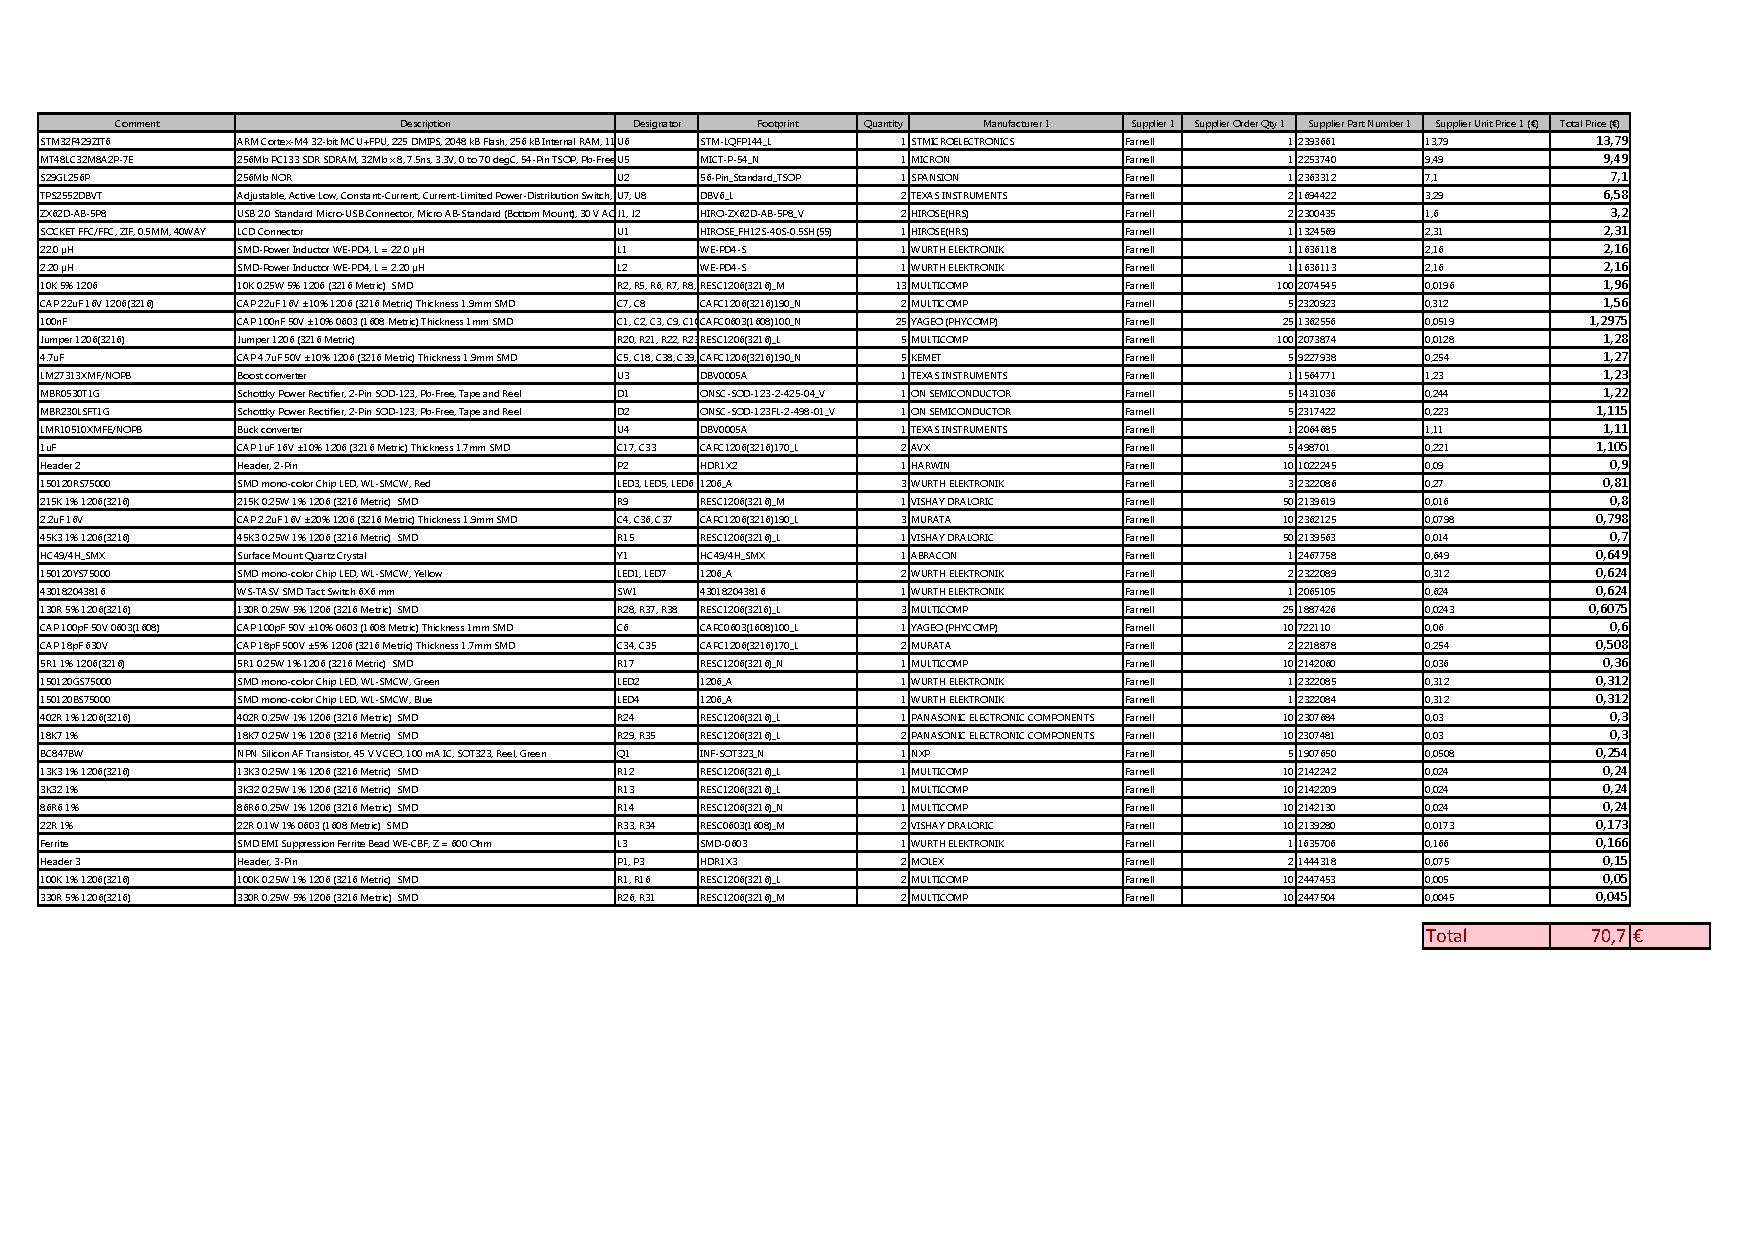
\includepdf[pages={1-}, link, linkname=Schematic, landscape=true]{PDF/PRT_STM32F429ZI_Eval-Board_BOM.pdf}